\documentclass[12pt]{extarticle}

% Language setting
% Replace `english' with e.g. `spanish' to change the document language
\usepackage[english]{babel}
% Useful packages
\usepackage{amsmath}
\usepackage{graphicx}
\usepackage[colorlinks=true, allcolors=blue]{hyperref}
\usepackage{ragged2e}
\usepackage{mathtools}
\usepackage{comment}
\usepackage{algorithm} 
\usepackage{algpseudocode} 
\usepackage{array}
\usepackage{hyperref}
\usepackage{float}
\usepackage{array,multirow}

\usepackage{titling}
\newcommand{\subtitle}[1]{%
  \posttitle{%
    \par\end{center}
    \begin{center}\large#1\end{center}
    \vskip0.5em}%
}


\newcommand\tab[1][1cm]{\hspace*{#1}}


\title{\centering{\huge{Subset Sum Problem in optimization form: a parallel approach}}}
\subtitle{\centering{Project for the GPU Computing course held by Professor Giuliano Grossi}, \\ \centering{University of Milan, February 2023}}
\author{Alessio La Greca}
\date{}

\usepackage[utf8]{inputenc}

\usepackage{geometry}
 \geometry{
 a4paper,
 total={160mm,250mm},
 left=20mm,
 top=20mm,
 }

\begin{document}

\maketitle

\begin{abstract}
The \emph{Subset Sum} with only positive values is a known problem in the field of computer science. The given input data is always:
\begin{itemize}
    \item a vector $A$ composed of $n$ positive values. This represents a \emph{multiset}, meaning that the same element can appear more than once;
    \item an objective value $c$.
\end{itemize}
In its basic form, the decision one, one is asked to tell whether there is a subset (which can as well be a sub-multiset) $A'$ of $A$ such that its elements, summed together, are equal to exactly $c$. This problem is known to be NP-complete. There is however an optimization form of the problem, where one is asked to find the value $c'$ such that:
\begin{itemize}
    \item $c'$ is given by the sum of the elements of a certain sub-multiset $A'$ of $A$;
    \item $c' \leq c$;
    \item There does not exist a value $c''$ given by a sub-multiset $A''$ of $A$ such that $c'' < c \land c'' > c'$.
\end{itemize}
Basically, we want to find the sub-multiset whose values, summed together, get as close as possible to $c$. This problem is regarded as NP-hard.
This particular problem, that will be of our complete interest throughout this report, and that we will simply call \emph{SSO} (\emph{SumsetSumOptimization}) from now on (as well as we'll call its decision form \emph{SSD} (\emph{SubsetSumDecision})), comes in handy in different applications. For example, this problem can be used in a \emph{Branch \& Bound} algorithm for solving the 3D Knapsack Problem, as a procedure for computing the dual bound of a partial solution.
There are different ways to tackle this problem: some give an exact result, while others use an heuristic approach. At the same time, different algorithms can be more or less efficient. Given that we'll focus only on \textbf{exact} algorithms, the goal of this report is to propose some procedures to solve the SSO problem by first studying sequential approaches, and then using parallel approaches to see what kind of speedup can be achieved. For the parallel algorithms, we'll leverage on a Nvidia GPU and its CUDA programming model.


\end{abstract}

{
  \hypersetup{linkcolor=black}
  \tableofcontents
}

\section{Introduction}
\subsection{Disclaimer}
Since the parallel algorithms are written in CUDA C, the reader shall be warned that some basic understanding of it is necessary to comprehend the implementation choices proposed in this report, altought the use of CUDA/Nvidia GPU specific features will be justified during the explaination of the relative algorithms. This means that an in-depth overview of things like the choice of the arrangement of the data in memory, the computations regarding thread indexes, and such, will be presented.\newline
The code relative to the algorithms proposed here can be found in the same repository in which this report lies\cite{website:repo}.
For further and deeper references, one can check the book\cite{cuda_c_programming:textbook} from which the CUDA C concepts used here have been learnt. We make the assumption that the reader is familiar with the basic CUDA terminology and concepts: each thread has a \emph{threadIdx}, \emph{blockIdx}, etc..
\subsection{Terminology}
From now on, we'll also refer informally to the vector of positive values, $A$, as \emph{volumes}, while the target value $c$ will be called \emph{capacity}. This is in analogy to the sub-procedure used in a \emph{Branch \& Bound} approach for the 3D Knapsack Problem. The volumes vector $A$ is considered to have lenght $n$, and it's a multiset, meaning that the same element can appear twice.\newline
Given for example five given items, their volumes vector of length $n=5$ would be:
\[A = \{2, 9, 9, 4, 7\}\]
Notice how the elements are not sorted nor in one way nor in the other. If not specified otherwise, we will assume that the order of the elements is not important, though \emph{sometimes having them sorted is necessary to have a correct algorithm.} Chapter \ref{GPU-exhaustive-section} will cover this in more detail.\newline
Another representation of the volumes vector is possible: in such case, if we assume that $m$ is the number of \emph{different} values we have at our disposal, we can build a representation of the multiset based on two vectors:
\begin{itemize}
    \item One is $A$, that this time contains only the different items. Considering the example shown before, we would have:
    \[A = \{2, 9, 4, 7\}\]
    \item The other is $B$, a vector that counts how many times an element of $A$ is present. In this case, it is:
    \[B = \{1, 2, 1, 1\}\]
\end{itemize}
In this report, we will always stick with the first of the two representations, but in the future also algorithms based on the second one could be used.
\subsection{Reference example}
\label{section-reference-example}
The main goal of this whole report is not to just show off some efficient code to solve this problem: also that, but it's also to study how one can approach a problem this hard through trial-and-error, refinement of different ideas and creativity, why not. In order to have a better grasp of what the algorithms are doing, a reference example can be useful. This is why we show here a toy instance that will be used to show the execution of the algorithm during their explanation. Note that sometimes we might need to show a more elaborated instance to better understand the algorithm, but unless differently stated, this one will be considered.\newline
Our \label{marker-toy-4-12} reference example has the following data:
\begin{itemize}
    \item $A = \{3, 5, 8, 10\}$
    \item $c = 12$
\end{itemize}
This instance will be called \emph{toy\_4\_12}, because $n = 4$ and $c = 12$. It's easy to see that this SSO instance has optimal value $11 = 3 + 8$. 

\subsection{Actual examples}
To compare the performance of the algorithms, however, some practical examples need to be used. In this section we present the instances we will be dealing with in this report.\newline
The first instance will be called \label{custom-1} \emph{custom\_1}, according to the function \emph{initialize\_custom\_1} (found in \emph{myProject/common.h}) called by the \emph{exec\_main\_0} command that can be found in the various makefile.

\begin{center}
\begin{tabular}{ | m{3cm} | m{2cm}|}
 \hline
 Volume value & Copies\\
 \hline
 1850000 & 2\\
 \hline
 120000 & 12\\
 \hline
 30000 & 10\\
 \hline
 1800 & 6\\
 \hline
 1250 & 4\\
 \hline
 400 & 2\\
 \hline
\end{tabular}
\end{center}
\begin{itemize}
     \item The total number of volumes is 36.
     \item The target capacity is 3690000.
     \item The best solution is 3606600.
 \end{itemize}
Here, we listed the volumes stating also their number of copies, instead of enumerating all of them explicitly. Please note that we did this just to make the instance clearer to read: the actual representation used by the algorithms will be the first one discussed before, that is, an array of 36 elements. The first two entries will be 1850000, the next twelve will be 120000, and so on.\newline
This instance should be thought as a meaningful one (that is, that could also be present in a real case scenario), althought relatively simple. We will use this mainly for the sequential algorithms.\newline
\newline
The second instance instead will be called \label{random-1} \emph{random\_1}, name given by the fact that we ask to an auxiliary procedure to randomly produce \emph{n} volumes within a given range, such that each of them is lower than the specified capacity. This instance, that can be launched from basically every makefile present in the repository, is the \emph{exec\_main\_1}, where the arguments (in their order of appearance) mean:
\begin{enumerate}
    \item 0: specifies that we want to use the auxiliary procedure for generating random volumes.
    \item 1: once again specifies that, in the auxiliary procedure, the volumes should be really randomly generated, and not taken from a pre-determined \emph{for} loop that would otherwise generate them.
    \item 100: the number of volumes we want for this instance.
    \item 1000000000: the capacity (one billion).
    \item 1: the seed for the random generation. This will ensure us that, althought the procedure randomly generates the volume values, they will always be the same for every execution.
\end{enumerate}
This instance, differently from the previous one, has no real meaning, and is such that actually the optimal solution requires to take all of the volumes. But, being it very large both in termis of \emph{n} and \emph{c}, it will be useful to compare fast GPU-based implementations.\newline
\newline
For each algorithm, we will execute each considered instance \textbf{five} times (if not specified otherwise), reporting the minimum, maximum and average time of execution. For the GPU, other profiling data could be presented.
\subsection{Used GPUs}
To test the parallel algorithms, the code was run on a Tesla T4 GPU, in which we were able to collect some metrics using Nsight compute CLI. The metrics that might appear are listed in the following table.
\begin{center}
\begin{tabular}{| m{5cm} | m{12cm}|}
 \hline
 Short name & Full metric name\\
 \hline
 Achieved occupancy & sm\_\_warps\_active.avg.pct\_of\_peak\_sustained\_active\\
 \hline
 Branch efficiency & smsp\_\_sass\_average\_branch\_targets\_threads\_uniform.pct\\
 \hline
 Global load efficiency & smsp\_\_sass\_average\_data\_bytes\_per\_sector\_mem\_global\_op\_ld.pct\\
 \hline
 Global store efficiency & smsp\_\_sass\_average\_data\_bytes\_per\_sector\_mem\_global\_op\_st.pct\\
 \hline
 Global load throughput & l1tex\_\_t\_bytes\_pipe\_lsu\_mem\_global\_op\_ld.sum.per\_second\\
 \hline
 Global store throughput & l1tex\_\_t\_bytes\_pipe\_lsu\_mem\_global\_op\_st.sum.per\_second\\
 \hline
 Dram read throughput & dram\_\_bytes\_read.sum.per\_second\\
 \hline
 Dram write throughput & dram\_\_bytes\_write.sum.per\_second\\
 \hline
 Shared efficiency & smsp\_\_sass\_average\_data\_bytes\_per\_wavefront\_mem\_shared.pct\\
 \hline
 Shared load throughput & l1tex\_\_data\_pipe\_lsu\_wavefronts\_mem\_shared\_op\_ld.sum.per\_second\\
 \hline
 Shared load transactions & l1tex\_\_data\_pipe\_lsu\_wavefronts\_mem\_shared\_op\_ld.sum\\
 \hline
 Shared store throughput & l1tex\_\_data\_pipe\_lsu\_wavefronts\_mem\_shared\_op\_st.sum.per\_second\\
 \hline
 Shared store transactions & l1tex\_\_data\_pipe\_lsu\_wavefronts\_mem\_shared\_op\_st.sum\\
 \hline
 Shared utilization & l1tex\_\_data\_pipe\_lsu\_wavefronts\_mem\_shared.avg.pct\_of\_peak\newline \_sustained\_elapsed\\
 \hline
 Shared load bank conflict & l1tex\_\_data\_bank\_conflicts\_pipe\_lsu\_mem\_shared\_op\_ld.sum\\
 \hline
 Shared store bank conflict & l1tex\_\_data\_bank\_conflicts\_pipe\_lsu\_mem\_shared\_op\_st.sum\\
 \hline
\end{tabular}
\end{center}
Depending on the implementation taken into account, only some metrics will be analyzed. We would like to give an additional description abuot some of them:
\begin{itemize}
    \item Global load/store throughput: the amount of data requested by instructions from/to the global address space. Includes transactions served by the L1 and L2 caches.
    \item Dram read/write througput: the amount of data requested by instructions from/to the global address space. It measures only the throughput between L2 and device memory.
\end{itemize}
Most of our applications run the same kernel multiple times (sometimes even thousands). The profiling tool gives, for each and every run, a full report about all the metrics asked. Reporting all of these metrics would be excessive and dispersive. In order to be concise, we decided to write down only the metrics of the first kernel launch, as all of them have the same global behaviour, and what changes is just some of the input data (a volume value, the content of a binary array...), without drastically affecting the overall performance.\newline
Sometimes, to test even further the code, we tried to run it also on another GPU, a GeForce RTX 3060, altought we weren't able to use profiling tools for that. This will still come in handy in some particular cases, to see if the same code run on a different hardware can give us better or worse performances.\newline
Lastly, note that the execution times reported for the GPU runs were measured using the CUDA events (scheduled on the default stream).

\section{CPU (Sequential) algorithms: exhaustive search}
\subsection{SSO: Exhaustive search}
\label{SSO-exhaustive-search}
The ol'good exhaustive approach, although obvious, is the first that must be presented, both to have a worst-case performance algorithm to which we'll compare the following ones, and to have a procedure that no matter what will give us the optimal value, which can then be used to make sure that the subsequent implementations are correct.\newline
The exhaustive search can be easily performed with a recursive algorithm. 
The algorithm produces all the $2^{n}$ strings of bit possible, where $n$ is the number of volumes. In a particular string of $n$ bits, let's call it $S$, we have $S[i] = 1$ if the \emph{i-th} element of the vector $A$ of volumes is considered in the current tentative solution, $0$ otherwise. The following table shows the tentative solutions produced for the \hyperref[marker-toy-4-12]{\emph{toy\_4\_12}} instance:
\begin{center}
\begin{tabular}{ | m{2cm} | m{5cm}| m{2cm} | m{2cm} |}
 \hline
 Bit string & Value & Feasible? & Optimal?\\
 \hline
 0000 & 0 + 0 + 0 + 0 = 0 & yes & no\\
 \hline
 0001 & 0 + 0 + 0 + 10 = 10 & yes & no\\
 \hline
 0010 & 0 + 0 + 8 + 0 = 8 & yes & no\\
 \hline
 0011 & 0 + 0 + 8 + 10 = 18 & no & no\\
 \hline
 0100 & 0 + 5 + 0 + 0 = 5 & yes & no\\
 \hline
 0101 & 0 + 5 + 0 + 10 = 15 & no & no\\
 \hline
 0110 & 0 + 5 + 8 + 0 = 13 & no & no\\
 \hline
 0111 & 0 + 5 + 8 + 10 = 23 & no & no\\
 \hline
 1000 & 3 + 0 + 0 + 0 = 3 & yes & no\\
 \hline
 1001 & 3 + 0 + 0 + 10 = 13 & no & no\\
 \hline
 1010 & 3 + 0 + 8 + 0 = 11 & yes & yes\\
 \hline
 1011 & 3 + 0 + 8 + 10 = 21 & no & no\\
 \hline
 1100 & 3 + 5 + 0 + 0 = 8 & yes & no\\
 \hline
 1101 & 3 + 5 + 0 + 10 = 18 & no & no\\
 \hline
 1110 & 3 + 5 + 8 + 0 = 16 & no & no\\
 \hline
 1111 & 3 + 5 + 8 + 10 = 26 & no & no\\
 \hline
\end{tabular}
\end{center}
The time complexity of this algorithm is $\Theta(2^{n})$, since all the possible solutions are visited. For the same reason, the space complexity of a recursive approach is $\mathcal{O}(n)$.
\subsection{SSO: Smarter exaustive search}
\label{SSO-smarter-exhaustive-search}
The exhaustive approach starts with an \emph{accum} variable, initialized to 0, that keeps track of the current sum produced do far. At each call, two recursive calls are made: in one, we add to the solution the next volume in $A$. In the other, we skip it. We can avoid visiting branches, in the recursion tree, that are made only of unfeasible solutions by saying, at a certain call:
\begin{itemize}
    \item If adding the current volume to the current partial solution does not exceed $c$, then both calls must be performed.
    \item But if it does, simply skip it: every solution that sums the current partial solution with this volume will be unfeasible.
\end{itemize}
This basically allows us to perform the exhaustive search only in the feasible region of the search space, since all the (partial) unfeasible solutions are immediately discarded. The following table shows the tentative solutions produced in this case:
\begin{center}
\begin{tabular}{ | m{2cm} | m{5cm}| m{2cm} |}
 \hline
 Bit string & Value & Optimal?\\
 \hline
 0000 & 0 + 0 + 0 + 0 = 0 & no\\
 \hline
 0001 & 0 + 0 + 0 + 10 = 10 & no\\
 \hline
 0010 & 0 + 0 + 8 + 0 = 8 & no\\
 \hline
 0100 & 0 + 5 + 0 + 0 = 5 & no\\
 \hline
 1000 & 3 + 0 + 0 + 0 = 3 & no\\
 \hline
 1010 & 3 + 0 + 8 + 0 = 11 & yes\\
 \hline
 1100 & 3 + 5 + 0 + 0 = 8 & no\\
 \hline
\end{tabular}
\end{center}
The time complexity of this algorithm is $\mathcal{O}(2^{n})$, since only in the worst case all the possible solutions are visited. The space complexity is $\mathcal{O}(n)$ once again.\newline
The code for this algorithm can be found in \emph{myProject/DIR\_\_\_CPU\_exhaustive\_opt}.\newline
Its performances are reported in the following table.
\begin{center}
\begin{tabular}{ | m{2.2cm} | m{2.2cm} | m{2.2cm} | m{2.2cm} |}
 \hline
 Instance & Min & Max & Avg\\
 \hline
 custom\_1 & 89.788956 s & 91.011294 s & 90.330596 s\\
 \hline

\end{tabular}
\end{center}
Actually, in an attempt to make the algorithm more efficient, we implemented it in a way that combines two approaches: a constructive and a destructive one. This came from an intuition: sometimes, instead of starting from the value 0 and ``enlarging'' it as close as possible to the target capacity, it can be better to start from the sum of all the volumes and removing some of them, until we reach a feasible solution.\newline
The algorithm proceeds as follows:
\begin{enumerate}
    \item Given the volumes, their number and the capacity, the mean volume is computed (the sum of all the volumes divided by their number).
    \item The capacity divided by this mean gives us an approximation of the number of volumes needed to fill the capacity. If this value is greater than half of the total number of volumes, the destructive approach is used. Otherwise, the constructive one is.
\end{enumerate}
This is an approach that is good in theory but can be arbitrarily bad in practice. Much depends on the distribution of the volumes and the capacity value. Still, it was necessary pointing out this implementation detail, that could be further addressed in the future. 

\section{CPU (Sequential) algorithms: Chad Parry's algorithm}
A completely different approach for solving the SSO problem comes from an algorithm proposed by Chad Parry\cite{website:chad-parry-algo}, where $b = c$:
\begin{figure}[htp]
    \centering
    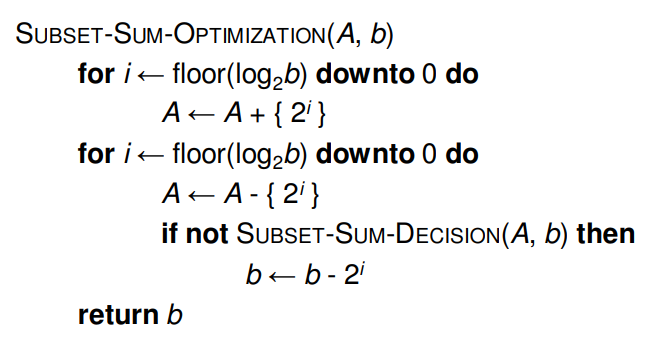
\includegraphics[width=14cm]{chad parry's algorithm.png}
    \caption{Chad Parry's Algorithm for the SubsetSumOptimization problem}
    \label{fig:chad-parry-algorithm}
\end{figure}\newline
The idea is first of all to enlarge the set of volumes with fictitious volumes that are all powers of 2, and then to solve multiple times the SSD problem in order to determine the optimal solution for the original SSO problem. This effectively reduces the SSO problem to the SSD problem, altought this must be solved multiple times. This means that if we can find an efficient way to solve the SSD problem, we automatically have an efficient way to solve the SSO problem. That said, we will now focus on different ways in which we can solve the SSD problem.
\subsection{Important premise}
Our main concern here is \textbf{efficiency}, or better \textbf{an efficient way to solve the SSO problem}.
Since Chad Parry's algorithm for the SSO problem relies on an iterated application of a procedure that solves the SSD problem, the overall complexity of the following algorithms is given by the complexity of the procedure that solves the SSD problem multiplied by the number of times that procedure is executed ($\lfloor log_2(c) \rfloor$).\newline
...and even so the computations wouldn't actually be precise, since each time the SSD procedure is executed, the input data are smaller than the previous execution (there is one less item): in short, to actually make an exact computational complexity study, we would need to consider all these things. But is it really necessary? We don't think so, since the only thing that we can manipulate in the Chad Parry's algorithm is the SSD procedure. We can easily see that, the more efficient this specific function is, the more the overall algorithm will be. So, we will focus on the time and space complexity of the proposed SSD procedure. 
\subsection{SSD: Exhaustive search}
Nothing stops us from taking the exhaustive approach used for the SSO problem in Section \ref{SSO-exhaustive-search} and use it to solve the decision form of the problem. The only difference is that this time we begin with the intention to fully explore the search space, by considering every possible string of $n$ bits, but, thanks to the short-circuit logic of the \emph{or} operator of the C language, we stop our search as soon as a solution equal to $c$ is found (otherwise, we fully explore the search space).\newline
The time complexity of this algorithm is $\mathcal{O}(2^{n})$, while the space complexity of a recursive approach is $\mathcal{O}(n)$.\newline
The code for this algorithm can be found in \emph{myProject/DIR\_\_\_CPU\_cp\_exhaustive\_dec}.\newline
In an attempt to run this algorithm to collect its performance on the 
\hyperref[custom-1]{\emph{custom\_1}} instance, the execution time exceeded 3 full hours, without coming to an end. The code is correct, and terminates giving the expected output for smaller instances: this one in particular, however, is way too big for it to be handled. This was to be expected since we basically repeat an exponential search multiple times. Let's than see how to address this problem.
\subsection{SSD: Dynamic Programming}
An exhaustive search is intrinsically inefficient: although such an algorithm can be used when the number of volumes is pretty low, as soon as this number rises a bit, the complexity becomes worse and worse. So, what we propose here is a Dynamic Programming approach to solve the SSD problem. Altough we could just present the most efficient algorithm we've found, we will instead show all the approaches we've come up with, for reasons stated in Section \ref{section-reference-example}.\newline
But before that, we need to state the general idea: a Dynamic Programming way to solve the SSD problem is to build a binary matrix DP with $n+1$ rows and $c+1$ columns, and to progressively fill each row, one after the other. Each cell of each row can be fully determined by at most two cells of the previous row.\newline
At row $i$ and column $j$, the cell DP[i][j] is \emph{true} if there exist a subset of the first $i$ items in $A$ that can sum up to $j$, \emph{false} otherwise. Note that the order of the elements in $A$ does not affect the final result.\newline
\begin{itemize}
    \item The first row covers the case in which no item is considered. This leads to an initial row that has the first element equal to \emph{true}, since summing no items gives 0, that fits exactly a capacity of 0, and \emph{false} for every other cell of the row, because without volumes we can't fill a positive capacity.
    \item Given any of the subsequent rows, we distinguish two cases:
    \begin{enumerate}
        \item $A[i] > j$, that is, the item $A[i]$ associated to the current row $i$ is greater than the current capacity $j$, so it can't possibly fit. In this case, we simply copy the previous case, since we can't do much else: $A[i] = A[i-1]$.
        \item $A[i] \leq j$. This time, item $A[i]$ fits in the capacity $j$, but this \emph{does not mean that it is part of the solution}. In fact, whether capacity $j$ was already reached without the support of this item (DP[i-1][j] = \emph{true}), adding it to the input data does not change the result. However, if instead DP[i-1][j] = \emph{false}, then we can try to see if the sub-problem of the row before that had capacity $j - A[i]$ admitted a postive answer, because if it did, then this does too. In short:\newline
        $DP[i][j] = DP[i-1][j] \lor DP[i-1][j-A[i]]$
    \end{enumerate}
\end{itemize}
By taking the element DP[n][c] (last row, last column), we can find out whether there is a positive answer to the original SSD problem or not.
\subsubsection{DP: Version 1}
The first implementation of this approach is extremely straightforward: just apply the algorithm as we have described it. We initialize the first row, and then compute all the following ones based on the one that precedes it. To do so, we need to allocate $n+1$ rows of length $c+1$ each. Since our code is developed in CUDA C, we could declare a row as an integer array. However, the type \emph{int} in C occupies 32 bits, which is a waste for just a binary information. This, together with the fact that there isn't a built-in \emph{boolean} type in C, led us to the choice of representing a cell of the matrix as an \emph{unsigned char}: it will be equal to 1 (\emph{true}) when the first $i$ objects admit a subset that sums up to $j$, 0 (\emph{false}) otherwise. This is because the unsigned char built-in type occupies just one byte of memory, the least amount of information a standard C variable can hold. The following table is the resulting matrix produced by this algorithm for the \hyperref[marker-toy-4-12]{\emph{toy\_4\_12}} instance.\newline
Actually, in order to be coherent with Chad Parry's algorithm, we should build multiple matrixes: one in which we consider the volumes given by the problem plus the fictitious volumes $\{8, 4, 2, 1\}$, then another with the same volumes except 8, and so on. However, to simplify the presentation of the concepts, since we just want to compare different SSD algorithms from an efficiency point of view, we'll just apply the DP algorithm to the decision version of the original \hyperref[marker-toy-4-12]{\emph{toy\_4\_12}} reference example.\newline
\begin{center}
\begin{tabular}{| m{0.6cm} | m{0.6cm}| m{0.6cm} | m{0.6cm} | m{0.6cm} | m{0.6cm} | m{0.6cm} | m{0.6cm} | m{0.6cm}| m{0.6cm} | m{0.6cm} | m{0.6cm} | m{0.6cm} | m{0.6cm} |}
 \hline
 & 0 & 1 & 2 & 3 & 4 & 5 & 6 & 7 & 8 & 9 & 10 & 11 & 12\\
 \hline
0 & T & F & F & F & F & F & F & F & F & F & F & F & F\\
\hline
3 & T & F & F & T & F & F & F & F & F & F & F & F & F\\
\hline
5 & T & F & F & T & F & T & F & F & T & F & F & F & F\\
\hline
8 & T & F & F & T & F & T & F & F & T & F & F & T & F\\
\hline
10 & T & F & F & T & F & T & F & F & T & F & T & T & F\\
\hline
\end{tabular}
\end{center}
Of course, the column index dictates the target capacity $c$ of the considered sub-problem, while the number at the beginning of each row represents the value of the new volume considered.\newline
The time complexity of this algorithm is $\Theta(n \times c)$ (to be precise it would be exactly $(n+1) \times (c+1)$), and the space complexity is exactly the same, since we allocated $n+1$ rows of $c+1$ elements each. Note that in this case the space complexity coincides exactly with the number of bytes used, since each cell is represented, in our CUDA C implementation, by an unsigned char.\newline
The code for this algorithm can be found in \emph{myProject/DIR\_\_\_CPU\_cp\_dp}, in the file \emph{CPU\_dp.cu}.\newline
Its performances are reported in the following table.
\begin{center}
\begin{tabular}{ | m{2.2cm} | m{2.2cm} | m{2.2cm} | m{2.2cm} |}
 \hline
 Instance & Min & Max & Avg\\
 \hline
 custom\_1 & 10.637604 s & 10.928177 s & 10.741072 s\\
 \hline
\end{tabular}
\end{center}
\subsubsection{DP: Version 2}
\label{CPU-dp-v2}
For a problem like this, it's not that difficult to have instances with a very high capacity. Even billions are totally common. If we consider that this high capacity value gets multiplied by the number of items, things get worse, both time-wise but most importantly space-wise. We say ``most importantly'' because, even though the time complexity is our main concern, if we don't have enough memory to solve the problem, we can't do much. And $\Theta(n \times c)$ bytes seem a lot, can't we do something better? Of course we can.\newline
Since every line other than the first is completely determined by the preceeding one, we can allocate just two rows:
\begin{enumerate}
    \item Initially, fill the first one as we know: \emph{true} in the first cell, \emph{false} in every other one.
    \item Set a variable $i = 0$, that represents the current number of items we are considering.
    \item Repeat the following steps until $i = n$ (every volume has been considered):
    \begin{enumerate}
        \item $i = i + 1$;
        \item Compute the second row from the first one, by considering only the first $i$ items;
        \item Overwrite the first row with the second.
    \end{enumerate}
\end{enumerate}
The following tables represent the subsequent states of the matrix throughout the execution of the algorithm on the \hyperref[marker-toy-4-12]{\emph{toy\_4\_12}} instance:
\begin{center}
\begin{tabular}{| m{0.6cm} | m{0.6cm}| m{0.6cm} | m{0.6cm} | m{0.6cm} | m{0.6cm} | m{0.6cm} | m{0.6cm} | m{0.6cm}| m{0.6cm} | m{0.6cm} | m{0.6cm} | m{0.6cm} | m{0.6cm} |}
 \hline
 & 0 & 1 & 2 & 3 & 4 & 5 & 6 & 7 & 8 & 9 & 10 & 11 & 12\\
 \hline
0 & T & F & F & F & F & F & F & F & F & F & F & F & F\\
\hline
3 &  &  &  &  &  &  &  &  &  &  &  &  & \\
\hline
\end{tabular}
\end{center}

\begin{center}
\begin{tabular}{| m{0.6cm} | m{0.6cm}| m{0.6cm} | m{0.6cm} | m{0.6cm} | m{0.6cm} | m{0.6cm} | m{0.6cm} | m{0.6cm}| m{0.6cm} | m{0.6cm} | m{0.6cm} | m{0.6cm} | m{0.6cm} |}
 \hline
 & 0 & 1 & 2 & 3 & 4 & 5 & 6 & 7 & 8 & 9 & 10 & 11 & 12\\
 \hline
0 & T & F & F & F & F & F & F & F & F & F & F & F & F\\
\hline
3 & T & F & F & T & F & F & F & F & F & F & F & F & F\\
\hline
\end{tabular}
\end{center}

\begin{center}
\begin{tabular}{| m{0.6cm} | m{0.6cm}| m{0.6cm} | m{0.6cm} | m{0.6cm} | m{0.6cm} | m{0.6cm} | m{0.6cm} | m{0.6cm}| m{0.6cm} | m{0.6cm} | m{0.6cm} | m{0.6cm} | m{0.6cm} |}
 \hline
 & 0 & 1 & 2 & 3 & 4 & 5 & 6 & 7 & 8 & 9 & 10 & 11 & 12\\
 \hline
3 & T & F & F & T & F & F & F & F & F & F & F & F & F\\
\hline
5 & T & F & F & T & F & T & F & F & T & F & F & F & F\\
\hline
\end{tabular}
\end{center}

\begin{center}
\begin{tabular}{| m{0.6cm} | m{0.6cm}| m{0.6cm} | m{0.6cm} | m{0.6cm} | m{0.6cm} | m{0.6cm} | m{0.6cm} | m{0.6cm}| m{0.6cm} | m{0.6cm} | m{0.6cm} | m{0.6cm} | m{0.6cm} |}
 \hline
 & 0 & 1 & 2 & 3 & 4 & 5 & 6 & 7 & 8 & 9 & 10 & 11 & 12\\
 \hline
5 & T & F & F & T & F & T & F & F & T & F & F & F & F\\
\hline
8 & T & F & F & T & F & T & F & F & T & F & F & T & F\\
\hline
\end{tabular}
\end{center}

\begin{center}
\begin{tabular}{| m{0.6cm} | m{0.6cm}| m{0.6cm} | m{0.6cm} | m{0.6cm} | m{0.6cm} | m{0.6cm} | m{0.6cm} | m{0.6cm}| m{0.6cm} | m{0.6cm} | m{0.6cm} | m{0.6cm} | m{0.6cm} |}
 \hline
 & 0 & 1 & 2 & 3 & 4 & 5 & 6 & 7 & 8 & 9 & 10 & 11 & 12\\
 \hline
8 & T & F & F & T & F & T & F & F & T & F & F & T & F\\
\hline
10 & T & F & F & T & F & T & F & F & T & F & T & T & F\\
\hline
\end{tabular}
\end{center}

The time complexity is unchanged, we still need $\Theta(n \times c)$ steps to compute the final result, but the memory now depends only on the value of $c$, and it's always $\Theta(2 \times c)$. One more thing to take into account, however, is the overhead caused by copying the second row into the first one at each step: from a practical point of view, it influences the overall time complexity of the procedure, making it worse then the previous version.\newline
The code for this algorithm can be found in \emph{myProject/DIR\_\_\_CPU\_cp\_dp}, in the file \emph{CPU\_dp.cu}.\newline
Its performances are reported in the following table.
\begin{center}
\begin{tabular}{ | m{2.2cm} | m{2.2cm} | m{2.2cm} | m{2.2cm} |}
 \hline
 Instance & Min & Max & Avg\\
 \hline
 custom\_1 & 15.786004 s & 16.290045 s & 15.973391 s\\
 \hline
\end{tabular}
\end{center}

\subsubsection{DP: Version 3}
With the last paragraph, we've seen an implementation that improves memory usage, but worsens time complexity because of the overhead brought by the copy operations. However, it allowed us to reason about one thing: to compute a row, only the previous one is necessary. We will now take this argument one step forward, improving both time and space complexity.\newline
It is true that row $i$ can be fully determined by row $i-1$. But what actually happens is that the $j$-th element of row $i$ depends only on two elements of row $i-1$: the $j$-th one and the $(j-A[i])$-th one. Or at least, this is true for every $j \geq A[i]$, at row $i$. This could suggest us that copying the first $A[i]$ elements of row $i-1$ into row $i$ is redundant.\newline
At the same time, up until now we've filled row $i$ starting from the leftmost element to the rightmost one. Nothing stops us from doing it also the other way round. But why doing so? Because in this way we no longer need two data structures to store the old and new row, and we can do everything in-place. This does not affect correctness. Each element is in fact dependent only on elements on its left. Given this, modifying in-place the contents of the array starting from the last element makes the array such that, at a certain step $i$, it can be divided into two parts:
\begin{itemize}
    \item A left one, composed of elements that consider only the first $i-1$ volumes. For each of these elements, it's true that the only entries necessary to compute the new value (the one that considers also the new $i$-th volume) are the element itself and the one $A[i]$ positions on its left.
    \item A right one, with elements that instead consider the first $i$ volumes. These values are already updated, and won't be used by any of the left part, since they only care about elements on their left.
\end{itemize}
So, we have found a procedure that needs always one row (an array of $c+1$ entries), and that does not have the overhead of copying elements, since every value update is done in-place. At the end, the result can be red in the last position fo the array. Given the \hyperref[marker-toy-4-12]{\emph{toy\_4\_12}} example, the following are the states of the array data structure of length $c+1$ during the execution of this algorithm. The red elements represent the values that have actually been computed, while the black one were not touched:

\begin{center}
\begin{tabular}{| m{0.6cm} | m{0.6cm}| m{0.6cm} | m{0.6cm} | m{0.6cm} | m{0.6cm} | m{0.6cm} | m{0.6cm} | m{0.6cm}| m{0.6cm} | m{0.6cm} | m{0.6cm} | m{0.6cm} | m{0.6cm} |}
 \hline
 & 0 & 1 & 2 & 3 & 4 & 5 & 6 & 7 & 8 & 9 & 10 & 11 & 12\\
 \hline
0 & \textcolor{red}{T} & \textcolor{red}{F} & \textcolor{red}{F} & \textcolor{red}{F} & \textcolor{red}{F} & \textcolor{red}{F} & \textcolor{red}{F} & \textcolor{red}{F} & \textcolor{red}{F} & \textcolor{red}{F} & \textcolor{red}{F} & \textcolor{red}{F} & \textcolor{red}{F}\\
\hline
\end{tabular}
\end{center}

\begin{center}
\begin{tabular}{| m{0.6cm} | m{0.6cm}| m{0.6cm} | m{0.6cm} | m{0.6cm} | m{0.6cm} | m{0.6cm} | m{0.6cm} | m{0.6cm}| m{0.6cm} | m{0.6cm} | m{0.6cm} | m{0.6cm} | m{0.6cm} |}
 \hline
 & 0 & 1 & 2 & 3 & 4 & 5 & 6 & 7 & 8 & 9 & 10 & 11 & 12\\
 \hline
3 & T & F & F & \textcolor{red}{T} & \textcolor{red}{F} & \textcolor{red}{F} & \textcolor{red}{F} & \textcolor{red}{F} & \textcolor{red}{F} & \textcolor{red}{F} & \textcolor{red}{F} & \textcolor{red}{F} & \textcolor{red}{F}\\
\hline
\end{tabular}
\end{center}

\begin{center}
\begin{tabular}{| m{0.6cm} | m{0.6cm}| m{0.6cm} | m{0.6cm} | m{0.6cm} | m{0.6cm} | m{0.6cm} | m{0.6cm} | m{0.6cm}| m{0.6cm} | m{0.6cm} | m{0.6cm} | m{0.6cm} | m{0.6cm} |}
 \hline
 & 0 & 1 & 2 & 3 & 4 & 5 & 6 & 7 & 8 & 9 & 10 & 11 & 12\\
 \hline
5 & T & F & F & T & F & \textcolor{red}{T} & \textcolor{red}{F} & \textcolor{red}{F} & \textcolor{red}{T} & \textcolor{red}{F} & \textcolor{red}{F} & \textcolor{red}{F} & \textcolor{red}{F}\\
\hline
\end{tabular}
\end{center}

\begin{center}
\begin{tabular}{| m{0.6cm} | m{0.6cm}| m{0.6cm} | m{0.6cm} | m{0.6cm} | m{0.6cm} | m{0.6cm} | m{0.6cm} | m{0.6cm}| m{0.6cm} | m{0.6cm} | m{0.6cm} | m{0.6cm} | m{0.6cm} |}
 \hline
 & 0 & 1 & 2 & 3 & 4 & 5 & 6 & 7 & 8 & 9 & 10 & 11 & 12\\
 \hline
8 & T & F & F & T & F & T & F & F & \textcolor{red}{T} & \textcolor{red}{F} & \textcolor{red}{F} & \textcolor{red}{T} & \textcolor{red}{F}\\
\hline
\end{tabular}
\end{center}

\begin{center}
\begin{tabular}{| m{0.6cm} | m{0.6cm}| m{0.6cm} | m{0.6cm} | m{0.6cm} | m{0.6cm} | m{0.6cm} | m{0.6cm} | m{0.6cm}| m{0.6cm} | m{0.6cm} | m{0.6cm} | m{0.6cm} | m{0.6cm} |}
 \hline
 & 0 & 1 & 2 & 3 & 4 & 5 & 6 & 7 & 8 & 9 & 10 & 11 & 12\\
 \hline
10 & T & F & F & T & F & T & F & F & T & F & \textcolor{red}{T} & \textcolor{red}{T} & \textcolor{red}{F}\\
\hline
\end{tabular}
\end{center}
The time complexity is $\mathcal{O}(n \times c)$, because this time we don't do exactly $c$ operations at each step, but a bit less, depending on the current volume. The space complexity is $\Theta(c)$, possibly the smallest it can be.\newline
The code for this algorithm can be found in \emph{myProject/DIR\_\_\_CPU\_cp\_dp}, in the file \emph{CPU\_dp.cu}.\newline
Its performances are reported in the following table.
\begin{center}
\begin{tabular}{ | m{2.2cm} | m{2.2cm} | m{2.2cm} | m{2.2cm} |}
 \hline
 Instance & Min & Max & Avg\\
 \hline
 custom\_1 & 7.230589 s & 7.449816 & 7.347593 s\\
 \hline
\end{tabular}
\end{center}
Of course, for instances with a very high $c$, we might still have memory problems, as we need to allocate $c$ bytes of memory for this approach, but this is the best we can do with a Dynamic Programming sequential approach. The next step will be to translate this idea in a parallel algorithm.
\section{GPU (Parallel) algorithms: Chad Parry's algorithm}
Chad Parry's algorithm for the SSO problem, as we've seen in the previous chapter, is composed of multiple applications of a SSD procedure, that is up to us to implement. The most efficient implementation (time-wise at least) that we have seen is the one based on Dynamic Programming. This particular implementation is interesting also because it consists of many independent and simple operations. While it's true that each row needs the previous one to compute its entries (so, the rows can't be computed in parallel, but sequentially), the entries themselves are completely independent one another, and just need at most two elements of the previous row. So, they can be computed in parallel.\newline
In a very abstract way, what each entry of row $i$ does to compute its value is:
\begin{algorithmic}
\If{$j < A[i]$} 
    \State $DP[i][j] = DP[i-1][j]$
\Else
    \State $DP[i][j] = DP[i-1][j] \lor DP[i-1][j-A[i]]$
\EndIf 
\end{algorithmic}
This is a very simple procedure, and as such we can think of a CUDA application in which we run $c+1$ threads, where each of them deals with a particular entry of the DP array. The entry it deals with can be computed using its $threadIdx$ and $blockIdx$. Both for simplicity and similarity, we can think to organize the threads in 1-dimensional blocks. This allows us to compute the thread index inside the grid (and so the element of the DP array it deals with) as $idx = blockIdx.x * blockDim.x + threadIdx.x$. That being said, we can no longer resort on using just one array of $c+1$ entries as we did in the 3rd version of the DP sequential implementation. This is because every element of row $i$ must read at most two elements of the previous row, that must be kept consistent throughout the computations of this new row. So, the space complexity of the following algorithms for solving the SSD with a Dynamic Programming approach will have a space complexity of $\Theta(2 \times c)$. Their differences will lie in the time complexity.\newline
The general scheme of the following algorithms is basically always the same:
\begin{enumerate}
    \item Allocate, on the GPU, two arrays of length $c+1$: let's call them \emph{row\_0} and \emph{row\_1}. \textbf{Once again, to avoid wasting memory, these will be \emph{unsigned char} arrays. This is something to keep in mind, expecially when we'll talk about shared memory.}
    \item Launch a first kernel, \emph{kernel\_a}, to initialize \emph{row\_0} as expected: \emph{true} as first element, \emph{false} for every other one.
    \item For $c$ times, launch a second kernel, \emph{kernel\_b}, that computes the $i$-th row from the $i-1$-th one. 
    \item Finally, retrieve the result from the last entry of the last row computed.
\end{enumerate}
Since the complexity of the initialization kernel \emph{kernel\_a} is insignificant compared to the iterated application of \emph{kernel\_b}, we will focus only on the implementation details of this last one (also because all the \emph{kernel\_a} implementations are actually more or less the same). Moreover, if up until now we've focused on the asymptotic notations of $\mathcal{O}$ and $\Theta$ to describe the performance of the algorithms, we will now instead examine their efficiency in CUDA terms.\newline
Once again, we won't give immediately the best algorithm achieved: we will examine different ideas, by evolving each of them when possible in order to understand how one can exploit all of the Nvidia GPU features to achieve better and better performances.
\subsection{SSD: Basic v1}
The first approach that we propose is very naive and inefficient, but its simplicity will allow us to correctly reason about how to improve it.\newline
We first allocate a total of three unsigned char arrays of length $c+1$:
\begin{itemize}
    \item The first is on the host.
    \item The second and the third, respectively \emph{row\_0} and \emph{row\_1}, are on the device.
\end{itemize}
After having initialized the host array with the starting values, we compute each following row as follows:
\begin{enumerate}
    \item We copy the content of the host array into \emph{row\_0};
    \item We run \emph{kernel\_b} that computes the new row, \emph{row\_1}, from \emph{row\_0};
    \item We copy the content of \emph{row\_1} into the host array, and repeat from point 1.
\end{enumerate}
In order to be a bit more efficient, at each iteration we check if the last element of the host array is \emph{true}: if it is, we don't need to compute the following rows and we can immediately return a positive outcome.\newline
The main drawback of this approach is that it makes a lot of copies from the host to the device and viceversa, worsening the overall performance. It's no secret that in CUDA programming the host-to-device and device-to-host data copy is an important bottleneck for many applications.\newline
The code for this algorithm can be found in \emph{myProject/DIR\_\_\_GPU\_cp\_dp}, in the file \emph{GPU\_dp\_basic.cu}.\newline
Its performances are reported in the following table. Since in CUDA an important factor is also the block dimension, from now on we will execute the algorithm with multiple block configurations and see how the performances change. The ones we chose are 128, 256, 512 and 1024, since are usually the most meaningful.
\begin{center}
\begin{tabular}{ | m{2.2cm} | m{3cm} | m{2.4cm} | m{2.4cm} | m{2.4cm} |}
 \hline
 Instance & Block dimension & Min & Max & Avg\\
 \hline
 custom\_1 & 128 & 1.710427 s & 1.843904 s & 1.760543 s\\
 \hline
 custom\_1 & 256 & 1.696415 s & 1.843320 s & 1.761409 s\\
 \hline
 custom\_1 & 512 & 1.808097 s & 1.891201 s & 1.843313 s\\
 \hline
 custom\_1 & 1024 & 1.721849 s & 1.870658 s & 1.789238 s\\
 \hline
 random\_1 & 128 & 922.991272 s & 922.991272 s & 922.991272 s\\
 \hline
 random\_1 & 256 & 932.092773 s & 932.092773 s & 932.092773 s\\
 \hline
 random\_1 & 512 & 925.151550 s & 925.151550 s & 925.151550 s\\
 \hline
 random\_1 & 1024 & 925.771912 s & 925.771912 s & 925.771912 s\\
 \hline
\end{tabular}
\end{center}
Please note that the \hyperref[random-1]{\emph{random\_1}} instance was run only once per block configuration. Given how poor its time is, it wouldn't make much sense to average five different runs to make sure that this apporoach is quite terrible.\newline
Despite the massive number of copies from host to device and viceversa, this kernel still performs very well with the \hyperref[custom-1]{\emph{custom\_1}} instance. But this is no surprise: we already stated how this is actually a very simple one. In fact, the limited capacity is such that not much data needs to be transfered, and not for many times either, since $n = 36$, which is a pretty low value. The same, however, cannot be said for the \hyperref[random-1]{\emph{random\_1}} instance, that instead requires to transfer many times (100) \textbf{a lot} of bytes (almost 1 GB, given the capacity of one billion). Moreover, please note that we purposefully made this instance such that the optimal value is strictly lower than the capacity. In this way, the algorithm won't stop midway during the execution returning a positive answer, but instead will have to compute exactly $n$ rows, which is the worst case scenario. From now on, during this chapter, we will focus on the \hyperref[random-1]{\emph{random\_1}} instance, since the \hyperref[custom-1]{\emph{custom\_1}} would give very little detail about the actual improvement of the following algorithms, given that its execution time is already so low. The random instance, instead, is solved \emph{so badly} from this implementation that it will be a good reference for the other proposed approaches.
\subsection{SSD: Basic v2}
The very first improvement we can come up with is one that doesn't perform so many memory operations from host to device and viceversa. After all, we don't really care bringing the intermediate rows to the host (except maybe for the last element that could be \emph{true}), we just care about (the last element of) the last one. So, what can be done?\newline
We could think of performing device to device memory copy operations, but this is rather similar to the approach seen in Section \ref{CPU-dp-v2}, which wasn't very efficient. To avoid unnecessary copy operations, we can just swap the roles of the two device arrays, \emph{row\_0} and \emph{row\_1}, when a new row needs to be computed. The overall algorithm would be as follows:
\begin{enumerate}
    \item Allocate on the device two arrays of $c+1$ unsigned char: our old and good \emph{row\_0} and \emph{row\_1};
    \item Initialize \emph{row\_0} with \emph{kernel\_a};
    \item label \emph{row\_0} as the ``\emph{old row}'', and \emph{row\_1} as the ``\emph{new row}'';
    \item For $n$ times, do:
    \begin{enumerate}
        \item Compute the \emph{new row} from the \emph{old row} using \emph{kernel\_b};
        \item Swap the \emph{old row} and \emph{new row} labels, so that the new one becomes the old one (for the next iteration) and viceversa;
        \item Check if the last element of the row just computed is \emph{true}, and if it is, stop the loop and return \emph{true}.
    \end{enumerate}
\end{enumerate}
In this way we never perform any copy at the cost of simply remembering which row is the old one and which is the new one.\newline
The code for this algorithm can be found in\newline \emph{myProject/DIR\_\_\_GPU\_cp\_dp/DIR\_\_\_GPU\_cp\_dp\_basic}, in the file \emph{GPU\_dp\_basic.cu}.\newline
Its performances are reported in the following table.
\begin{center}
\begin{tabular}{ | m{2.2cm} | m{3.2cm} | m{2.2cm} | m{2.2cm} | m{2.2cm} |}
 \hline
 Instance & Block dimension & Min & Max & Avg\\
 \hline
 random\_1 & 128 & 51.836765 s & 53.753044 s & 52.907434 s\\
 \hline
 random\_1 & 256 & 52.563198 s & 52.636547 s & 52.600974 s\\
 \hline
 random\_1 & 512 & 52.629414 s & 53.146851 s & 53.033184 s\\
 \hline
 random\_1 & 1024 & 55.418789 s & 55.465378 s & 55.436583 s\\
 \hline
 \end{tabular}
 \end{center}
 While some metrics collected can be found in the following table.
\begin{center}
\noindent%
\resizebox{\textwidth}{!}{%
\begin{tabular}{ | m{2cm} | m{1.3cm} | m{2.2cm} | m{2.2cm} | m{2.2cm} | m{2.2cm} | m{1.9cm} | m{2.1cm} | m{1.9cm} | m{1.9cm} |}
 \hline
 Instance & Block dimension & Dram read throughput & Dram write throughput & Global load throughput & Global store throughput & Achieved occupancy & Branch efficiency & Global ld. efficiency & Global st. efficiency\\
 \hline
 random\_1 & 128 & 58.09 GB/s & 26.51 GB/s & 67.69 GB/s & 22.80 GB/s & 83.94\% & 100.00\% & 66.70\% & 100.00\%\\
 \hline
 random\_1 & 256 & 57.62 GB/s & 26.57 GB/s & 67.01 GB/s & 22.52 GB/s & 83.00\% & 100.00\% & 66.70\% & 100.00\%\\
 \hline
 random\_1 & 512 & 56.96 GB/s & 25.80 GB/s & 65.26 GB/s & 21.92 GB/s & 82.13\% & 100.00\% & 66.70\% & 100.00\%\\
 \hline
 random\_1 & 1024 & 54.13 GB/s & 24.79 GB/s & 61.40 GB/s & 20.67 GB/s & 90.06\% & 100.00\% & 66.70\% & 100.00\%\\
 \hline
 \end{tabular}%
}
\end{center}
Althought the best performances are reached with the second configuration, the highest occupancy is given by the fourth one, which instead gives the worst performance. This apparent contraddiction is probably explained by the overall throughput, that is higher in the first two configurations.\newline
Please also note that the following sections of this chapter will start from this implementation, trying to improve it with different CUDA features.
\subsection{SSD: Unrolling}
The \emph{unrolling} is a common technique in CUDA programming, that aims to improve the performance of kernels. The main idea is to take a for loop performed in a thread, and reduce the number of times it is executed by writing its body multiple times. This has two major advantages:
\begin{itemize}
    \item We have a reduced instruction overhead, because the maintenance operations ($i < x; i$++) are performed less times.
    \item If the unrolled body now contains independent memory load/store operations, these can be scheduled simultaneously by the hardware, as memory latency can be better hidden.
\end{itemize}
That being said, the unrolling doesn't need to have a loop to start with. The idea is generally implemented by saying: take a thread and make it perform multiple independent operations. In our case, this is absolutely doable: each thread can handle the computation of $k$ values for row $i$, instead of just one. This reduces by a factor $k$ the overall number of threads needed, and increments the number of operations each thread must perform. However, being these memory independent operations, our hope is to achieve a speedup thanks to the fact that these will be scheduled efficiently and simultaneously by the scheduler.\newline
The only (human) problem are the indexes: we must sort out, for each thread, the $k$ indexes of the elements of row $i$ that must be computed, but in such a way that each thread handles $k$ elements that are different from those associated to every other thread. Now, given this constraint, generally speaking these indexes can be chosen arbitrarily. However, in order to be efficient, the accesses made to the global memory (where \emph{row\_0} and \emph{row\_1} lie) should be \textbf{\emph{aligned}} and \textbf{\emph{coalesced}}.\newline
In the CUDA programming model, 32 threads with consecutive indexes work in a \emph{SIMT} fashion to achieve parallelism, and they are collectively called \emph{warp}. This affects the way instructions and memory operations are performed. In particular, when the threads of a warp want to access global memory, they group together their \emph{individual requested addresses} into one \emph{memory access request}. This memory access request is serviced in one or more \textbf{\emph{memory transactions}}, that can be seen as the ``currency'' for any global memory access request. The less memory transactions a memory access request needs to be satisfied, the more efficient the access becomes.\newline
Now, a memory transaction can be either of 128-bytes or 32-bytes, depending on whether the L1 on-chip cache is used or not. The important thing to note is that \textbf{these bytes are always contiguous} and \textbf{their initial address is always a multiple of 128 or 32}. To service even a memory access to just one byte, at least 32 consecutive bytes need to be read. This is why a memory access request should be composed of individual requested addresses that are \emph{aligned} and \emph{coalesced}, because in this way the number of necessary memory transactions is reduced. 
\begin{itemize}
    \item \emph{Aligned} means that the first individual address requested by a warp is an even multiple of 32 or 128, respectively the granularity of the L2 device cache or L1 on-chip cache.
    \item \emph{Coalesced} means that all the addresses requested by the threads of the warp are contiguous.
\end{itemize}
When both these assumptions hold for a memory request, we can be sure that the access will be efficient. The most common case is the one in which the threads of a warp read one integer each (4 bytes), and these bytes are such that:
\begin{itemize}
    \item The first address is an even multiple of 32/128;
    \item All of them are adjacent in memory (for example, they are consecutive elements of an integer array).
\end{itemize}
Depending on the particular application, enabling the L1 cache can provide better performance or not. However, talking about our specific problem: we have had threads that don't read 4 bytes each, but one byte each. We have to take this into account when reasoning about how to arrange the memory indexes to these threads when performing the unrolling.
\subsubsection{Unrolling factor 8}
Let's then try to implement the unrolling approach to our kernels. To do that, we first have to choose an \emph{unrolling factor}, that in this case translates to the value of $k$, that is how many elements of the new row a thread should compute. We first propose the value $k = 8$, since it's a pretty standard one.\newline
Once again, after \emph{row\_0} has been initialized, we can modify the structure of \emph{kernel\_b} in such a way that each thread deals with 8 consecutive elements of the new row.\newline
Each thread computes its first index as:
\[idx = blockIdx.x * blockDim.x * 8 + threadIdx.x * 8 \]
and obtains the seven following ones by summing 1, 2, $\dots$, 7 do \emph{idx}. Each of these threads reads the corresponding value of the previous row and if necessary the one that is $A[i]$ positions before that. In this way, the 32 threads of a warp issue a collective memory request of 256 or 512 bytes to the global memory, such that:
\begin{itemize}
    \item The index of the first address is always a multiple of 256, that is both a multiple of 32 and 128, so the access is aligned.
    \item All these bytes are contiguous, which means that the access is also coalesced.
\end{itemize}
The code for this algorithm can be found in\newline \emph{myProject/DIR\_\_\_GPU\_cp\_dp/DIR\_\_\_GPU\_cp\_dp\_uroll}, in the file \emph{GPU\_dp\_uroll.cu}.\newline
Its performances are reported in the following table.
\begin{center}
\begin{tabular}{ | m{2.2cm} | m{3.2cm} | m{2.2cm} | m{2.2cm} | m{2.2cm} |}
 \hline
 Instance & Block dimension & Min & Max & Avg\\
 \hline
 random\_1 & 128 & 30.193602 s & 31.185658 s & 30.785120 s\\
 \hline
 random\_1 & 256 & 30.713205 s & 31.206713 s & 30.914854 s\\
 \hline
 random\_1 & 512 & 30.879026 s & 31.026178 s & 30.950231 s\\
 \hline
 random\_1 & 1024 & 31.786615 s & 32.058788 s & 31.909336 s\\
 \hline
 \end{tabular}
 \end{center}
 While some metrics collected can be found in the following table.
\begin{center}
\noindent%
\resizebox{\textwidth}{!}{%
\begin{tabular}{ | m{2cm} | m{1.3cm} | m{2.3cm} | m{2.2cm} | m{2.3cm} | m{2.3cm} | m{1.9cm} | m{2.1cm} | m{1.9cm} | m{1.9cm} |}
 \hline
 Instance & Block dimension & Dram read throughput & Dram write throughput & Global load throughput & Global store throughput & Achieved occupancy & Branch 
 \newline efficiency & Global ld. efficiency & Global st. efficiency\\
 \hline
 random\_1 & 128 & 135.78 GB/s & 41.71 GB/s & 597.63 GB/s & 282.02 GB/s & 90.30\% & 100.00\% & 11.77\% & 12.50\%\\
 \hline
 random\_1 & 256 & 136.53 GB/s & 41.84 GB/s & 602.38 GB/s & 284.19 GB/s & 89.27\% & 100.00\% & 11.77\% & 12.50\%\\
 \hline
 random\_1 & 512 & 137.49 GB/s & 41.98 GB/s & 605.49 GB/s & 285.63 GB/s & 88.25\% & 100.00\% & 11.77\% & 12.50\%\\
 \hline
 random\_1 & 1024 & 122.70 GB/s & 39.39 GB/s & 571.21 GB/s & 269.29 GB/s & 93.46\% & 100.00\% & 11.77\% & 12.50\%\\
 \hline
 \end{tabular}%
}
\end{center}
As expected, the unrolling provided, thanks to multiple independent memory operations, a drastic increase in the throughput, granting a considerable speedup.
In this case, the use of L1 cache can improve a bit the overall performances. To see that, run first the application with the L1 cache enabled (using \emph{-Xptxas -dlcm=ca}), then run again with it disabled (using \emph{-Xptxas -dlcm=cg}). The results reported used, of course, the L1 cache.
\subsubsection{Unrolling factor 16}
The improved performances of the last kernel suggest us to try to push even further the unrolling factor. Let's then try to set $k=16$. This time, each thread computes its first index as
\[idx = blockIdx.x * blockDim.x * 16 + threadIdx.x * 16 \]
and the fifteen following ones by summing 1, 2, $\dots$, 15 to \emph{idx}. The logic behind this implementation is unchanged with respect to the preceeding one.\newline
The code for this algorithm can be found in\newline \emph{myProject/DIR\_\_\_GPU\_cp\_dp/DIR\_\_\_GPU\_cp\_dp\_uroll}, in the file \emph{GPU\_dp\_uroll.cu}.\newline
Its performances are reported in the following table.
\begin{center}
\begin{tabular}{ | m{2.2cm} | m{3.2cm} | m{2.2cm} | m{2.2cm} | m{2.2cm} |}
 \hline
 Instance & Block dimension & Min & Max & Avg\\
 \hline
 random\_1 & 128 & 50.806286 s & 51.642052 s & 51.376543 s\\
 \hline
 random\_1 & 256 & 50.801529 s & 50.929413 s & 50.864144 s\\
 \hline
 random\_1 & 512 & 50.560051 s & 50.679070 s & 50.636001 s\\
 \hline
 random\_1 & 1024 & 51.771023 s & 51.802116 s & 51.790547 s\\
 \hline
 \end{tabular}
 \end{center}
 While some metrics collected can be found in the following table.
\begin{center}
\noindent%
\resizebox{\textwidth}{!}{%
\begin{tabular}{ | m{2cm} | m{1.3cm} | m{2.3cm} | m{2.2cm} | m{2.3cm} | m{2.3cm} | m{1.9cm} | m{2.1cm} | m{1.9cm} | m{1.9cm} |}
 \hline
 Instance & Block dimension & Dram read throughput & Dram write throughput & Global load throughput & Global store throughput & Achieved occupancy & Branch 
 \newline efficiency & Global ld. efficiency & Global st. efficiency\\
 \hline
 random\_1 & 128 & 69.62 GB/s & 21.35 GB/s & 587.07 GB/s & 285.78 GB/s & 95.02\% & 100.00\% & 6.07\% & 6.25\%\\
 \hline
 random\_1 & 256 & 69.34 GB/s & 21.26 GB/s & 585.09 GB/s & 284.81 GB/s & 93.84\% & 100.00\% & 6.07\% & 6.25\%\\
 \hline
 random\_1 & 512 & 69.92 GB/s & 21.52 GB/s & 592.00 GB/s & 288.16 GB/s & 93.72\% & 100.00\% & 6.07\% & 6.25\%\\
 \hline
 random\_1 & 1024 & 66.24 GB/s & 21.13 GB/s & 573.93 GB/s & 279.36 GB/s & 95.97\% & 100.00\% & 6.07\% & 6.25\%\\
 \hline
 \end{tabular}%
}
\end{center}
However, this time we didn't have an improvement, but instead a worsening. Althought the occupancy slightly increases, the main difference lies in the dram read and write throughput, that is basically halved with respect to the urolling 8. This might be caused by an excessive cache miss, due to the high number of data asked by each thread. 
\subsection{SSD: Shared Memory}
Another CUDA feature that allows programmers to achieve potential speedup in their applications is a program-managed, on-chip (so, per-Streaming Multiprocessor) cache. It is known as \emph{Shared Memory} (SMEM), and it shares the same on-chip physical memory of the L1 cache. For this reason only, load/store operations performed by a thread to the SMEM are much faster than those performed towards the global memory. However, to fully exploit its capabilities, one must know how data are organized and accessed in this memory.\newline
When designing a kernel, a certain amount of Shared Memory can be declared, either statically or dynamically. During the execution, each \emph{block} of the kernel has a certain amount of SMEM associated to it. This is an important point because the SMEM serves also as an intra-block communication mechanism. This means that threads of the same block can see and manage the same Shared Memory (the name \emph{shared} it's not random), but have no access whatsoever to that of any other thread block. This has two consequences:
\begin{itemize}
    \item Given that a single Streaming Multiprocessor can host multiple blocks at the same time, one should know how much SMEM can be given to a block in order not to affect the performances of the application. If a block requires a lot of SMEM, the hardware, that will associate that block to a SM, will also reserve enough Shared Memory for it, possibly preventing other blocks to be allocated on that same SM because of a lack of SMEM.
    \item When designing a Shared Memory based application, the programmer should reason about what the individual blocks of the grid will do, and how the threads will access to the SMEM.
\end{itemize}
The last point is particularly important because of the fact that the Shared Memory is organized in \emph{Memory Banks}. Basically, the entire Shared Memory can be divided into 32 parts, or banks. When a warp issues a SMEM load/store request, this results more or less efficient depending on (once again) the number of memory transactions needed to satisfy such request. In general, the SMEM is organized in rows, and each row is composed of 32 $\times$ 4 bytes, where every 4 consecutive bytes, called \emph{word}, belong to the same bank (some architectures enlarge the bank width up to 8, althought this does not change the principles explained here). If a warp SMEM access is such that \textbf{at most} one word per bank is requested, then the memory request is said to be conflictless, and just one memory transaction is necessary to satisfy the overall request. This is the case every programmer should strive to achieve. Of course, a conflictless access to the Shared Memory is possible when the memory word requested are aligned (with respect to the shared memory rows) and coalesced, but in general, the important part consists in building a memory access pattern such that it is conflictless.\newline

In our proposed implementation, each block requires \emph{blockDim.x} $\times$ 2 bytes of Shared Memory. In this way, every thread can move inside of it the two elements of the previous row necessary to compute the new one. If a thread is such that $idx < A[i]$, just $A[i-1]$ is copied in the SMEM. The actual address in which an element is copied depends on the \emph{warp index} and the \emph{thread index} of the current thread. The warp index is computed as
\[threadIdx.x / 32\]
while the thread index is simply \emph{threadIdx.x}.\newline
Each warp uses 64 contiguous bytes of memory. The main operations performed are:
\begin{enumerate}
    \item Load from the global memory the $idx$-th and (in case) the ($idx - A[i]$)-th elements of the previous row, storing their values in the Shared Memory. Each warp uses the bytes that range from index $warp\_id \times 64$ included to $(warp\_id + 1) \times 64$ excluded, so that no data is overwritten during the lifetime of a kernel.
    \item Then, the two values are read from the Shared Memory and put inside two local variables. If one element is not available, it is simply set to \emph{false}.
    \item Finally, the value for the $idx$-th entry is computed as $a \lor b$ and brought back to global memory.
\end{enumerate}
Since each warp writes and reads a chunk of 64 contiguous bytes from the Shared Memory, with its starting index being a multiple of 64, the access is always coalesced and aligned, and can be satisfied with only one memory transaction.\newline
The code for this algorithm can be found in\newline \emph{myProject/DIR\_\_\_GPU\_cp\_dp/DIR\_\_\_GPU\_cp\_dp\_smem}, in the file \emph{GPU\_dp\_smem.cu}.\newline
Its performances are reported in the following table.
\begin{center}
\begin{tabular}{ | m{2.2cm} | m{3.2cm} | m{2.2cm} | m{2.2cm} | m{2.2cm} |}
 \hline
 Instance & Block dimension & Min & Max & Avg\\
 \hline
 random\_1 & 128 & 51.365772 s & 51.723152 s & 51.538487 s\\
 \hline
 random\_1 & 256 & 51.338116 s & 51.758690 s & 51.523809 s\\
 \hline
 random\_1 & 512 & 54.096416 s & 54.631626 s & 54.312395 s\\
 \hline
 random\_1 & 1024 & 61.635738 s & 62.138893 s & 61.804496 s\\
 \hline
 \end{tabular}
 \end{center}
 While some metrics collected can be found in the following table.
\begin{center}
\noindent%
\resizebox{\textwidth}{!}{%
\begin{tabular}{ | m{2cm} | m{1.3cm} | m{2.2cm} | m{2.2cm} | m{2.2cm} | m{2.2cm} | m{1.9cm} | m{2.1cm} | m{1.9cm} | m{1.9cm} |}
 \hline
 Instance & Block dimension & Dram read throughput & Dram write throughput & Global load throughput & Global store throughput & Achieved occupancy & Branch efficiency & Global ld. efficiency & Global st. efficiency\\
 \hline
 random\_1 & 128 & 74.89 GB/s & 35.11 GB/s & 88.58 GB/s & 30.02 GB/s & 77.90\% & 100.00\% & 66.70\% & 100.00\%\\
 \hline
 random\_1 & 256 & 73.39 GB/s & 33.98 GB/s & 85.58 GB/s & 28.87 GB/s & 76.90\% & 100.00\% & 66.70\% & 100.00\%\\
 \hline
 random\_1 & 512 & 71.03 GB/s & 31.47 GB/s & 78.82 GB/s & 26.68 GB/s & 75.13\% & 100.00\% & 66.70\% & 100.00\%\\
 \hline
 random\_1 & 1024 & 65.07 GB/s & 27.37 GB/s & 65.83 GB/s & 22.80 GB/s & 84.72\% & 100.00\% & 66.70\% & 100.00\%\\
 \hline
 \end{tabular}%
}
\end{center}
The metrics regarding the shared memory specifically are reported here:
\begin{center}
\begin{tabular}{ | m{2cm} | m{2cm} | m{3cm} | m{3cm} |}
 \hline
 Instance & Block\newline dimension & Shared load\newline bank conflicts & Shared store\newline bank conflicts\\
 \hline
 random\_1 & 128 & 0 & 1,121,338\\
 \hline
 random\_1 & 256 & 0 & 1,086,880\\
 \hline
 random\_1 & 512 & 0 & 1,131,275\\
 \hline
 random\_1 & 1024 & 0 & 3,877,240\\
 \hline
 \end{tabular}
\end{center}
We clearly have something strange here. The execution times reported are as bad as the ones of the basic v2 version, if not worse. But one could argue that this is due to the apparently enormous amount of Shared Memory bank conflicts during the storing operations. Now, this would actually make sense... if it wasn't for the fact that, after some hours of testing, we found out what was causing all these conflicts. It was not the way the data were organized in the shared memory, but instead, it was just one line of code:
\begin{center}
    CHECK(cudaDeviceSetCacheConfig(cudaFuncCachePreferShared));
\end{center}
In fact, after commenting this line of code, we obtained the following results. Pay attention specifically to the third table, that reports the bank conflicts: they have now disappeared.
\begin{center}
\begin{tabular}{ | m{2.2cm} | m{3.2cm} | m{2.2cm} | m{2.2cm} | m{2.2cm} |}
 \hline
 Instance & Block dimension & Min & Max & Avg\\
 \hline
 random\_1 & 128 & 51.003735 s & 53.052624 s & 52.472406 s\\
 \hline
 random\_1 & 256 & 52.623817 s & 53.271679 s & 52.848441 s\\
 \hline
 random\_1 & 512 & 55.497005 s & 55.944008 s & 55.722385 s\\
 \hline
 random\_1 & 1024 & 63.210556 s & 63.763607 s & 63.462196 s\\
 \hline
 \end{tabular}
 \end{center}
\begin{center}
\noindent%
\resizebox{\textwidth}{!}{%
\begin{tabular}{ | m{2cm} | m{1.3cm} | m{2.2cm} | m{2.2cm} | m{2.2cm} | m{2.2cm} | m{1.9cm} | m{2.1cm} | m{1.9cm} | m{1.9cm} |}
 \hline
 Instance & Block dimension & Dram read throughput & Dram write throughput & Global load throughput & Global store throughput & Achieved occupancy & Branch efficiency & Global ld. efficiency & Global st. efficiency\\
 \hline
 random\_1 & 128 & 74.89 GB/s & 35.11 GB/s & 88.60 GB/s & 30.03 GB/s & 77.90\% & 100.00\% & 66.70\% & 100.00\%\\
 \hline
 random\_1 & 256 & 73.39 GB/s & 33.99 GB/s & 85.60 GB/s & 28.88 GB/s & 76.86\% & 100.00\% & 66.70\% & 100.00\%\\
 \hline
 random\_1 & 512 & 70.61 GB/s & 31.30 GB/s & 78.40 GB/s & 26.54 GB/s & 75.20\% & 100.00\% & 66.70\% & 100.00\%\\
 \hline
 random\_1 & 1024 & 64.70 GB/s & 27.22 GB/s & 65.47 GB/s & 22.68 GB/s & 84.78\% & 100.00\% & 66.70\% & 100.00\%\\
 \hline
 \end{tabular}%
}
\end{center}
\begin{center}
\begin{tabular}{ | m{2cm} | m{2cm} | m{3cm} | m{3cm} |}
 \hline
 Instance & Block\newline dimension & Shared load\newline bank conflicts & Shared store\newline bank conflicts\\
 \hline
 random\_1 & 128 & 0 & 0\\
 \hline
 random\_1 & 256 & 0 & 0\\
 \hline
 random\_1 & 512 & 0 & 0\\
 \hline
 random\_1 & 1024 & 0 & 0\\
 \hline
 \end{tabular}
\end{center}
This is actually even stranger, because:
\begin{itemize}
    \item The only way in which the bank conflicts could be explained in the first case is that the data, before being brought into the shared memory, get carried into the L1 cache, that is subject to many misses because of the on-chip memory preference set to the Shared one. Still, it doesn't sound like a very convincing argument.
    \item Apparently, even if the difference is small, having zero conflicts results in a slightly longer execution time.
\end{itemize}
We could study other metrics to try to explain this strange phenomena. But in the last section of this chapter, where we'll run the code on the GeForce RTX 3060 GPU, we'll see that instead the Shared Memory actually brings an advantage.\newline
These results leave us with a moral dilemma: should we use the incriminated line of code in the following kernels that use the Shared Memory, having better executions times but more conflicts, or should we delete it, so as to remove all the bank conflicts and theoretically have a more scalable application, in spite of longer execution times? We decided to go for the second way. The absence of bank conflicts can't possibly be a bad thing, and the execution times are not that different regardless. So, keep in mind that, in every kernel that follows using Shared Memory, we will always have zero conflicts.
\subsection{SSD: Unrolling 8 + Shared Memory}
So far in this chapter, the unrolling technique with unrolling factor $k = 8$ and the Shared Memory brought us the best speedup (for the SMEM, this is true only with the GeForce RTX 3060 GPU) to the standard Dynamic Programming parallel (v2) approach. It comes natural to think that merging these two approaches can give us even better performaces. Let's see if that's true.\newline
With the Shared Memory approach, each thread had to bring into the on-chip cache at most two bytes from the previous row. In total, a warp managed 64 bytes of the SMEM.\newline
In the unrolling approach with factor $k = 8$, each thread had to read up to 16 bytes from the previous row, in order to determine 8 new values. Basically, each warp managed 16 $\times$ 32 = 512 bytes.\newline
Combining these approaches, we would have threads that bring 16 bytes of data from global memory to the Shared Memory, for a total of \emph{blockDim.x} $\times$ 2 $\times$ 8 bytes of SMEM necessary for each block. Each warp still manages 512 bytes in total, so a minimum of four rows of SMEM are necessary to contain them. If these bytes are coalesced and aligned in the Shared Memory, exactly four rows need to be accessed by a warp to fulfill a memory request.\newline
All that remains is to decide how to organize these data into the Shared Memory. Since a SMEM row is made of 32 $\times$ 4 = 128 bytes, and at most 512 bytes are read by a warp, we can organize the application in the following way:
\begin{enumerate}
    \item Each warp of a block is given a contiguous set of 512 SMEM bytes, with the starting one being an even multiple of 512. This guarantees us that the accesses to the memory are coalesced and aligned.
    \item A given thread has an index \emph{idx = blockIdx.x * blockDim.x * 8 + threadIdx.x * 8}, that tells which is the first element of the new row that it must compute. The other ones are obtained by summing to \emph{idx} the values 1, 2, $\dots$, 7. Each of these indexes allow us to go to the previous row and read up to two values:
    \begin{itemize}
        \item The one of the same index;
        \item The one of the same index minus $A[i]$, if that index is a valid one.
    \end{itemize}
    These 16 values are read from the global memory and stored in the shared one, and each group of four is in a different row.
    \item The bytes written in the SMEM are then brought in some local arrays (one for each thread), \emph{a} and \emph{b}, of lenght 8.
    \item For $i = 0 \dots 7$, we compute the new row's value of position $idx + i$ as
    \[a[i] \lor b[i]\]
    and store it into the global memory.
\end{enumerate}
The code for this algorithm can be found in\newline \emph{myProject/DIR\_\_\_GPU\_cp\_dp/DIR\_\_\_GPU\_cp\_dp\_uroll8\_smem}, in the file \emph{GPU\_dp\_uroll8\_smem.cu}.\newline
Its performances are reported in the following table.
\begin{center}
\begin{tabular}{ | m{2.2cm} | m{3.2cm} | m{2.2cm} | m{2.2cm} | m{2.2cm} |}
 \hline
 Instance & Block dimension & Min & Max & Avg\\
 \hline
 random\_1 & 128 & 35.535706 s & 36.506088 s & 36.030728 s\\
 \hline
 random\_1 & 256 & 36.008530 s & 36.347065 s & 36.143403 s\\
 \hline
 random\_1 & 512 & 36.322014 s & 36.610592 s & 36.480317 s\\
 \hline
 random\_1 & 1024 & 39.713650 s & 39.971500 s & 39.865581 s\\
 \hline
 \end{tabular}
 \end{center}
 While some metrics collected can be found in the following table.
\begin{center}
\noindent%
\resizebox{\textwidth}{!}{%
\begin{tabular}{ | m{2cm} | m{1.3cm} | m{2.3cm} | m{2.2cm} | m{2.3cm} | m{2.3cm} | m{1.9cm} | m{2.1cm} | m{1.9cm} | m{1.9cm} |}
 \hline
 Instance & Block dimension & Dram read throughput & Dram write throughput & Global load throughput & Global store throughput & Achieved occupancy & Branch efficiency & Global ld. efficiency & Global st. efficiency\\
 \hline
 random\_1 & 128 & 150.47 GB/s & 47.87 GB/s & 681.94 GB/s & 321.81 GB/s & 71.79\% & 100.00\% & 11.77\% & 12.50\%\\
 \hline
 random\_1 & 256 & 150.21 GB/s & 47.33 GB/s & 675.33 GB/s & 318.63 GB/s & 70.51\% & 100.00\% & 11.77\% & 12.50\%\\
 \hline
 random\_1 & 512 & 151.61 GB/s & 46.57 GB/s & 665.67 GB/s & 314.02 GB/s & 75.90\% & 100.00\% & 11.77\% & 12.50\%\\
 \hline
 random\_1 & 1024 & 112.15 GB/s & 35.68 GB/s & 515.51 GB/s & 243.06 GB/s & 80.35\% & 100.00\% & 11.77\% & 12.50\%\\
 \hline
 \end{tabular}%
}
\end{center}
Once again, the Shared Memory seems to ``bring down'' the performances, while the unrolling still grants us a good speedup. The overall result is better than the base case, but worse than the unrolling 8 one.
\subsection{Results on the GeForce RTX 3060}
The following table shows the results obtained by running all the algorithms on our GeForce RTX 3060 GPU. The instance used is always \hyperref[random-1]{\emph{random\_1}}, and given the results obtained in the last experiments, we will fix the block size at 256, which seems to give the best overall results. Also, since as we've seen the execution times tend to not change so much, we run each approach just once.
\begin{center}
\begin{tabular}{ | m{3.2cm} | m{3.2cm} |}
 \hline
 Approach & Execution time\\
 \hline
 Basic v2 & 40.223137 s\\
 \hline
 uroll8 & 28.227880 s\\
 \hline
 uroll16 & 53.374401 s\\
 \hline
 smem & 38.298553 s\\
 \hline
 uroll8 + smem & 20.191149 s\\
 \hline
 \end{tabular}
 \end{center}
As stated before, the Shared Memory here seems to provide a meaningful speedup, expecially when paired with the unrolling.
\section{GPU (Parallel) algorithms: exhaustive search}
\label{GPU-exhaustive-section}
The approach seen in the previous chapter is extremely good, but has one unsolvable problem: the memory limit. In order for the Dynamic Programming parallel approach to work, in fact, we need to allocate $(c + 1) \times 2$ bytes on the device global memory. If the instance is such that the capacity is greater than half the total size of the global memory, this approach cannot be used. However, one approach that didn't have any memory problem was the exhaustive one (since its space complexity was $\mathcal{O}(n)$). Althought intrinsically inefficient time-wise, it has no rivals space-wise. So, we could think of a parallel implementation of this approach.\newline
Recursion in cuda is possible thanks to Dynamic Parallelism. In Dynamic Parallelism, a kernel's thread is able to launch a nested grid of thread blocks, and as such can be used to implement recursive functions. However, due to the limits of Dynamic Parallelism-based kernels, such as the maximum nested grid's depth, and the general complexity of designing a scalable application based on this feature, we won't rely on it to implement an exhaustive parallel search.
\subsection{The abstract idea}
What are we actually doing when performing an exhaustive search? Given the volumes and their number, \emph{n}, we are taking, one by one, all the elements from the powerset of the volumes set, and for each of them we compute its value (given by the sum of the volumes considered). If we are lucky and smart enough, we can a priori exclude some of these sets because we recognize their unfeasibility. We did exactly this with the sequential exhaustive approach, where we cut the recursive exploration as soon as the capacity was exceeded.\newline
An idea we came up with for a parallel approach is, in a very abstract way:
\begin{enumerate}
    \item Partition the search space, given by $2^{n}$ elements, into subsets.
    \item For each of them, find out if it \emph{could} contain the optimal solution or not.
    \item If it could, examine it exaustively. Otherwise, skip it.
\end{enumerate}
To make up an algorithm from this idea, we have to answer two questions:
\begin{enumerate}
    \item How should we partition the search space?
    \item How can we find out if a subset \textbf{surely does NOT contain} the optimal solution?
\end{enumerate}
\subsection{The abstract algorithm}
In order to answer in an effective way these questions, we have to describe what we actually want to do in our code. To do so, we have many different intuitions hat need to be exposed.
\subsubsection{Intuition 1}
Given that our search space is the powerset of the set of volumes, how can we explicitly represent and identify one of its elements (a tentative solution, a subset of the volumes set)? In the sequential implementation, the solutions were generated implicitly: when the bottom of the recursion was reached, the \emph{accum} variable held all the volumes considered by the solution generated, and so, indirectly, also the ignored volumes. But in this case we want to explicitly say, in a tentative solution: ``this volume is part of the sum; this other volume is not; this one more is part of the solution'', etc.. How can we do that?\newline
Since the presence or absence of a volume in a solution is a binary information, one bit will suffice. Therefore, given an \emph{a priori ordering of the volumes, such that it won't ever be changed}, we can represent a tentative solution as a binary string of length $n$. Its $i-$th bit will be 1 if the $i-$th element of the ordering is present in the solution, 0 otherwise. The question now becomes: \emph{which ordering should we use?} An arbitrary one, or something more elaborated?
\subsubsection{Intuition 2}
When we deal with the binary representation of positive numbers, we have an interesting property: \emph{the rightmost bits refer to lower powers of two, while the leftmost ones refer to higher powers of two}. More generally, we can say that the rightmost bits represent lower values, while the leftmost ones represent higher values. Reasoning by analogy, we can decide to order the volumes in a decreasing way. First, we'll have the largest, represented by the leftmost bits of the binary representation of a solution. In the last positions, we'll have the smallest, represented by the rightmost bits of the binary string. \emph{But does this particular bit string representation give us any advantage?}
\subsubsection{The ``Binary Decreasing'' representation}
Yes, it does! So, generally speaking, when we are presented with a Subset Sum Optimization problem instance, where we have $n$ volumes in total in an array called $A$, we can sort this array in decreasing order, and start visiting (with basicaly a \emph{constructive approach}) the search space by generating all the binary strings associated to $A$ in the usual order.\newline
The important thing to note is an interesting property of the bit strings generated in this way: \textbf{if we partition the search space of the bit strings in contiguous chunks, where}:
\begin{itemize}
    \item \textbf{The chunk size is always a fixed power of 2};
    \item \textbf{The first index of each chunk is an even multiple of the chosen chunk dimension;}
\end{itemize}
\textbf{then we are sure that, for each chunk, its \emph{minimum} value is the very first, and the \emph{maximum} value is the last one}. In this way, if the chosen power of 2 is $p$, we have partitioned the search space into $2^{n} / p$ subsets, and some of them don't need to be explored, as we can find out immediately if they \emph{might} contain the optimal solution or they \emph{surely} don't. If the first element of the subset is lower or equal than the capacity value, then that subset contains for sure at least one feasible solution (the first one, or the minimum for that chunk), and as such must be explored. \textbf{But}, if instead the first value is greater than the capcity, then the subset contains only unfeasible solutions, since that first value is the minimum for that chunk.
\newline
Let's see an example of this. Suppose we have an instance with:
\begin{itemize}
    \item $n = 6$
    \item $A = [5, 3, 5, 7, 3, 5]$
\end{itemize}
The first thing to do is to order $A$ in decreasing order. In this way, we have $A = [7, 5, 5, 3, 3, 3]$. The following table reports all the tentative solutions for this instance, specifying their bit string, the elements that correspond to it, and the actual value. The latter columns show how dividing the search space in contiguous chunks of power of 2 elements makes each chunk such that the first element is the minimum, while the last is the maximum (there isn't any ``Distance 2'' column as it would have been identical to the ``Value'' column).
\begin{center}
\begin{tabular}{ | m{1.5cm} | m{1.7cm} | m{3cm} | m{1.2cm} | m{1.3cm} | m{1.3cm} | m{1.5cm} | m{1.5cm} |}
 \hline
 Index (base 2) & Index (base 10) & Subset sum & Value & Dist. 4 & Dist. 8 & Dist. 16 & Dist. 32\\
 \hline
 0 & 000000 & 0+0+0+0+0+0 & 0 & 0                  & 0                     & 0                   & 0\\
 \cline{1-4}
 1 & 000001 & 0+0+0+0+0+3 & 3 & \multirow{2}{*}{ } & \multirow{6}{*}{ }    & \multirow{14}{*}{}  & \multirow{30}{*}{}\\
 \cline{1-4}
 2 & 000010 & 0+0+0+0+3+0 & 3 &                    &                       &                     &\\
 \cline{1-4}
 3 & 000011 & 0+0+0+0+3+3 & 6 &                  6 &                       &                     &\\
 \cline{1-5}
 4 & 000100 & 0+0+0+5+0+0 & 5 &                  5 &                       &                     &\\
 \cline{1-4}
 5 & 000101 & 0+0+0+5+0+3 & 8 & \multirow{2}{*}{ } &                       &                     &\\
 \cline{1-4}
 6 & 000110 & 0+0+0+5+3+0 & 8 &                    &                       &                     &\\
 \cline{1-4}
 7 & 000111 & 0+0+0+5+3+3 & 11 &                11 & 11                    &                     &\\
 \cline{1-6}

 8 & 001000 & 0+0+5+0+0+0 & 5 & 5                  & 5                     &                     &\\
 \cline{1-4}
 9 & 001001 & 0+0+5+0+0+3 & 8 & \multirow{2}{*}{ } & \multirow{6}{*}{ }    &                     &\\
 \cline{1-4}
 10 & 001010 & 0+0+5+0+3+0 & 8 &                   &                       &                     &\\
 \cline{1-4}
 11 & 001011 & 0+0+5+0+3+3 & 11 &               11 &                       &                     &\\
 \cline{1-5}
 12 & 001100 & 0+0+5+5+0+0 & 10 &               10 &                       &                     &\\
 \cline{1-4}
 13 & 001101 & 0+0+5+5+0+3 & 13 & \multirow{2}{*}{ } &                     &                     &\\
 \cline{1-4}
 14 & 001110 & 0+0+5+5+3+0 & 13 &                    &                     &                     &\\
 \cline{1-4}
 15 & 001111 & 0+0+5+5+3+3 & 16 &                 16 & 16                  & 16                  &\\
 \cline{1-7}

 16 & 010000 & 0+5+0+0+0+0 & 5 &                    5 & 5                  & 5                   &\\
 \cline{1-4}
 17 & 010001 & 0+5+0+0+0+3 & 8 & \multirow{2}{*}{ }   & \multirow{6}{*}{ } & \multirow{14}{*}{}  &\\
 \cline{1-4}
 18 & 010010 & 0+5+0+0+3+0 & 8 &                      &                    &                     &\\
 \cline{1-4}
 19 & 010011 & 0+5+0+0+3+3 & 11 &                  11 &                    &                     &\\
 \cline{1-5}
 20 & 010100 & 0+5+0+5+0+0 & 10 &                  10 &                    &                     &\\
 \cline{1-4}
 21 & 010101 & 0+5+0+5+0+3 & 13 & \multirow{2}{*}{ }  &                    &                     &\\
 \cline{1-4}
 22 & 010110 & 0+5+0+5+3+0 & 13 &                     &                    &                     &\\
 \cline{1-4}
 23 & 010111 & 0+5+0+5+3+3 & 16 &                  16 & 16                 &                     &\\
 \cline{1-6}

 24 & 011000 & 0+5+5+0+0+0 & 10 &                  10 & 10                 &                     &\\
 \cline{1-4}
 25 & 011001 & 0+5+5+0+0+3 & 13 & \multirow{2}{*}{ }   & \multirow{6}{*}{ } &                    &\\
 \cline{1-4}
 26 & 011010 & 0+5+5+0+3+0 & 13 &                      &                    &                    &\\
 \cline{1-4}
 27 & 011011 & 0+5+5+0+3+3 & 16 &                   16 &                    &                    &\\
 \cline{1-5}
 28 & 011100 & 0+5+5+5+0+0 & 15 &                   15 &                    &                    &\\
 \cline{1-4}
 29 & 011101 & 0+5+5+5+0+3 & 18 & \multirow{2}{*}{ }   &                    &                    &\\
 \cline{1-4}
 30 & 011110 & 0+5+5+5+3+0 & 18 &                      &                    &                    &\\
 \cline{1-4}
 31 & 011111 & 0+5+5+5+3+3 & 21 &                   21 & 21                 & 21                 & 21\\
 \cline{1-8}

 32 & 100000 & 7+0+0+0+0+0 & 7 &                      7 & 7                 & 7                  & 7\\
 \cline{1-4}
 33 & 100001 & 7+0+0+0+0+3 & 10 & \multirow{2}{*}{ }    & \multirow{6}{*}{ } & \multirow{14}{*}{} & \multirow{30}{*}{}\\
 \cline{1-4}
 34 & 100010 & 7+0+0+0+3+0 & 10 &                       &                    &                    &\\
 \cline{1-4}
 35 & 100011 & 7+0+0+0+3+3 & 13 &                    13 &                    &                    &\\
 \cline{1-5}
 36 & 100100 & 7+0+0+5+0+0 & 12 &                    12 &                    &                    &\\
 \cline{1-4}
 37 & 100101 & 7+0+0+5+0+3 & 15 & \multirow{2}{*}{ }    &                    &                    &\\
 \cline{1-4}
 38 & 100110 & 7+0+0+5+3+0 & 15 &                       &                    &                    &\\
 \cline{1-4}
 39 & 100111 & 7+0+0+5+3+3 & 18 &                    18 & 18                 &                    &\\
 \cline{1-6}

 40 & 101000 & 7+0+5+0+0+0 & 12 &                    12 & 12                 &                    &\\
 \cline{1-4}
 41 & 101001 & 7+0+5+0+0+3 & 15 & \multirow{2}{*}{ }    &                    &                    &\\
 \cline{1-4}
 42 & 101010 & 7+0+5+0+3+0 & 15 &                       &                    &                    &\\
 \cline{1-4}
 43 & 101011 & 7+0+5+0+3+3 & 18 &                    18 &                    &                    &\\
 \cline{1-5}
 44 & 101100 & 7+0+5+5+0+0 & 17 &                    17 &                    &                    &\\
 \cline{1-4}
 45 & 101101 & 7+0+5+5+0+3 & 20 & \multirow{2}{*}{ }    &                    &                    &\\
 \cline{1-4}
 46 & 101110 & 7+0+5+5+3+0 & 20 &                       &                    &                    &\\
 \cline{1-4}
 47 & 101111 & 7+0+5+5+3+3 & 23 &                    23 & 23                 & 23                 &\\
 \cline{1-7}

 \end{tabular}
 \end{center}


 \begin{center}
\begin{tabular}{ | m{1.5cm} | m{1.7cm} | m{3cm} | m{1.2cm} | m{1.3cm} | m{1.3cm} | m{1.5cm} | m{1.5cm} |}
\cline{1-7}
 48 & 110000 & 7+5+0+0+0+0 & 12 &                     12 & 12                 & 12                 &\\
 \cline{1-4}
 49 & 110001 & 7+5+0+0+0+3 & 15 & \multirow{2}{*}{ }     & \multirow{6}{*}{ } & \multirow{14}{*}{} & \multirow{30}{*}{}\\
 \cline{1-4}
 50 & 110010 & 7+5+0+0+3+0 & 15 &                        &                    &                    &\\
 \cline{1-4}
 51 & 110011 & 7+5+0+0+3+3 & 18 &                     18 &                    &                    &\\
 \cline{1-5}
 52 & 110100 & 7+5+0+5+0+0 & 17 &                     17 &                    &                    &\\
 \cline{1-4}
 53 & 110101 & 7+5+0+5+0+3 & 20 & \multirow{2}{*}{ }     &                    &                    &\\
 \cline{1-4}
 54 & 110110 & 7+5+0+5+3+0 & 20 &                        &                    &                    &\\
 \cline{1-4}
 55 & 110111 & 7+5+0+5+3+3 & 23 &                     23 & 23                 &                    &\\
 \cline{1-6}

 56 & 111000 & 7+5+5+0+0+0 & 17 &                     17 & 17                 &                    &\\
 \cline{1-4}
 57 & 111001 & 7+5+5+0+0+3 & 20 & \multirow{2}{*}{ }     & \multirow{6}{*}{ } &                    &\\
 \cline{1-4}
 58 & 111010 & 7+5+5+0+3+0 & 20 &                        &                    &                    &\\
 \cline{1-4}
 59 & 111011 & 7+5+5+0+3+3 & 23 &                     23 &                    &                    &\\
 \cline{1-5}
 60 & 111100 & 7+5+5+5+0+0 & 22 &                     22 &                    &                    &\\
 \cline{1-4}
 61 & 111101 & 7+5+5+5+0+3 & 25 & \multirow{2}{*}{ }     &                    &                    &\\
 \cline{1-4}
 62 & 111110 & 7+5+5+5+3+0 & 25 &                        &                    &                    &\\
 \cline{1-4}
 63 & 111111 & 7+5+5+5+3+3 & 28 &                     28 & 28                 & 28                 & 28\\
 \cline{1-8}
 \end{tabular}
 \end{center}

 \subsubsection{Data representation and the general algorithm}
 Provided that the Binary Decreasing representation is how we want to describe our data at an abstract level, we now have to punctualize the corresponding code implementation for such data. Given the array of volumes (immediately sorted in decreasing order), the integer values $n$ and $c$, and a $jump$ value, that is a power of 2 and represents the size of a chunk, we will build a char array of length $n$ that will represent the current solution. Let's call this array, as well as the binary representation of the solution it holds, \emph{global\_index\_counter}. At an abstract level, the algorithm used to apply this exhaustive search works as follows:
 \begin{enumerate}
     \item Generate a bit string of $n$ bits set to 0, and save this value in the \emph{global\_index\_counter}.
     \item Take the $jump$ integer value and convert it into its binary form using exactly $n$ bits.
     \item Initialize a variable, \emph{final\_result}, to 0. This variable will progressively hold the best solution found so far.
     \item For $2^{n} / jump$ times, repeat:
    \begin{enumerate}
        \item If the solution represented by the current value of \emph{global\_index\_counter} is unfeasible, skip directly to step g) (we basically skip the current chunk as it only contains unfeasible solutions).
        \item Launch a kernel that will compute, in parallel, all the solutions from \emph{global\_index\_counter} (included) to \emph{global\_index\_counter} + $jump$ (excluded). The feasible solutions produced by this kernel are then collected in an array.
        \item Launch a reduction kernel that will take the maximum value out of the array produced during the last step.
        \item Execute one last reduction on the CPU. The value obtained in this way, let's call it $s$, is the best feasible solution of the current chunk.
        \item If $s > final\_solution$, update \emph{final\_solution} with $s$.
        \item Optionally (althought there is no reason not to perform this operation) check if \emph{final\_result} is equal to $c$. If it is, terminate the algorithm, as the optimal solution is exactly $c$.
        \item \emph{global\_index\_counter} = \emph{global\_index\_counter} + $jump$.
    \end{enumerate}
    \item Return \emph{final\_result}.
 \end{enumerate}
 One might argue that we could have represented the index of the current solution in base 10 (an integer) and not in base 2 (a binary array). After all, it's easy to convert a base 10 number into its binary representation, and as such find out which are the elements to take into account for the current solution. But using an integer index would limit us once again, as the maximum value that an $int$ variable can hold is $2^{32}$ or $2^{64}$ if we are using a \emph{long int}. This would limit the maximum number of input volumes to 32 or 64. Instead, the \emph{char array} representation doesn't give any limit to the number of possible volumes (well technically \emph{it does}, as the memory is limited for whatever hardware, but the point is that even having 1000 distinct volumes would simply imply to use a 1000 byte array, which is very simple to allocate and manage. Basically, the $int$ data type gives us a strict upper bound on the number of indexes we can manage, while the \emph{char array} doesn't).\newline
 The operations stated above are performed by a collection of functions that can be found in each \emph{GPU\_exhaustive\_opt\_common.cu} file. These files are found in each directory inside the \emph{DIR\_\_\_GPU\_exhaustive\_opt/DIR\_\_\_GPU\_exhaustive\_opt\_constructive} directory, which is also the place in which all the following implementations proposed in this chapter lie. Each implementation might change a bit their code, but the main behaviour is always the same:
 \begin{itemize}
     \item \emph{produce\_initial\_string}: creates a char array of length $n$ with all zeros.
     \item \emph{add\_bit\_strings}: given two binary strings of the same length, this function sums them, storing the result in the first argument.
     \item \emph{convert\_to\_binary}: converts an integer number into a binary char arrray of length $n$. Little trivia: originally, the function used an \emph{if} statement to determine whether the current bit value had to be 0 or 1. This was later changed into one line of code \textbf{(res[i] = ((char) k\&1) + '0';)} that doesn't involve conditional statements, thus avoiding warp divergence.
     \item \emph{equal\_bit\_strings}: checks whether two bit strings are the same or not.
     \item \emph{value\_of\_solution}: takes a bit string of length $n$, as well as the volumes array, and gives the corresponding Subset Sum value of that solution.
 \end{itemize}
 Some of the functions stated above are marked with the \emph{\_\_host\_\_ \_\_device\_\_} qualifiers, so that they can be called both by the host code and device code.
 \subsection{Jump value}
 The \emph{jump} value determines how big is the kernel launched, if it is launched in the first place. Generally speaking, this value should be neither too low nor too high. If too low, the kernels launched would be very small, possibly achieving small occupancy, and we would have a lot of overhead due to the large number of control operations of the main \emph{for} loop. If too large, we risk to partition the search space in regions that contain many unfeasible solutions alongside few feasible ones. This is bad, because we are then forced to compute a lot of useless solutions to consider just a minority of feasible ones. In the benchmarks that follows, the value will be always set to $2^{24}$, which seemed reasonable to us.
 \subsection{The reduction kernel}
 The reduction kernel used is adapted by the one present in the CUDA C programming book\cite{cuda_c_programming:textbook}, and therefore its performances won't be stated here. The only difference is that instead of performing a sum of the input elements, it returns the maximum value. Note that it uses both the unrolling technique as well as the Shared Memory, making it extremely efficient.
 
\subsection{SSO: Basic}
The first implementation we propose is the CUDA C code transposition of the pesudo-code we gave earlier.\newline
The code for this algorithm can be found in the files contained in the directory\newline \emph{myProject/DIR\_\_\_GPU\_exhaustive\_opt/DIR\_\_\_GPU\_exhaustive\_opt\_constructive/\newline DIR\_\_\_GPU\_exhaustive\_opt\_basic}. Its performances are reported in the following table.
\begin{center}
\begin{tabular}{ | m{2.2cm} | m{3.2cm} | m{2.2cm} | m{2.2cm} | m{2.2cm} |}
 \hline
 Instance & Block dimension & Min & Max & Avg\\
 \hline
 random\_1 & 128 & 38.313484 s & 39.111614 s & 38.743160 s\\
 \hline
 random\_1 & 256 & 38.455868 s & 38.611488 s & 38.542525 s\\
 \hline
 random\_1 & 512 & 38.506222 s & 38.720413 s & 38.577960 s\\
 \hline
 random\_1 & 1024 & 43.258228 s & 43.423359 s & 43.313046 s\\
 \hline
 \end{tabular}
 \end{center}
 While some metrics collected can be found in the following table.
\begin{center}
\noindent%
\resizebox{\textwidth}{!}{%
\begin{tabular}{ | m{2cm} | m{1.3cm} | m{2.3cm} | m{2.3cm} | m{2.3cm} | m{2.3cm} | m{1.9cm} | m{2.1cm} | m{1.9cm} | m{1.9cm} |}
 \hline
 Instance & Block dimension & Dram read throughput & Dram write throughput & Global load throughput & Global store throughput & Achieved occupancy & Branch 
 \newline efficiency & Global ld. efficiency & Global st. efficiency\\
 \hline
 random\_1 & 128 & 9.98 GB/s & 107.54 GB/s & 70.29 GB/s & 3.90 GB/s & 94.43\% & 100.00\% & 12.50\% & 156.25\%\\
 \hline
 random\_1 & 256 & 9.96 GB/s & 108.68 GB/s & 71.02 GB/s & 3.95 GB/s & 90.06\% & 100.00\% & 12.50\% & 156.25\%\\
 \hline
 random\_1 & 512 & 9.57 GB/s & 101.13 GB/s & 67.06 GB/s & 3.73 GB/s & 92.88\% & 100.00\% & 12.50\% & 156.25\%\\
 \hline
 random\_1 & 1024 & 15.26 GB/s & 92.19 GB/s & 58.16 GB/s & 3.23 GB/s & 97.10\% & 100.00\% & 12.50\% & 156.25\%\\
 \hline
 \end{tabular}%
}
\end{center}
\subsection{Other approaches}
We also tried five more approaches to improve the base implementation:
\begin{enumerate}
    \item \emph{Constant Memory}: since the volumes don't change during the execution, we made a variant that stores them in the Constan Memory of the device.
    \item \emph{Unroll}: since in this application there are many for loop, we tried to unroll some of them with an unrolling factor of 8.
    \item \emph{Smem}: each thread needs to read the same starting binary index from the global memory, which then modifies it in-place to obtain its effective index. We decided to import the starting index in the Shared Memory, since every thread of a block needs to access it.
    \item \emph{Unroll and Constant Memory}: the combination of the Unrolling and the Constant variants.
    \item \emph{Unrolling, Constant and Shared Memory}: the combination of all the variants.
\end{enumerate}
Sadly, none of these implementations gave us noticeable speedups, so we won't report here their performances, as they are extremely similar to the ones of the basic approach. This might be due to the fact that the main core of the application lies in a \emph{for} loop performed by the host, which implicitly sets a bound to the speedup we can achieve. Moreover, the partitions of the search space are visited sequentially, and if there are many unfeasible regions that divide two feasible ones, many idle iterations could delay the start of the execution of the next kernel. 
\section{Future directions}
While for the Chad Parry's algorithm we examinated in a satisfying way many approaches (althought the Tesla T4 GPU still hides some secrets, with its whacky Shared Memory...), there is still margin of improvement for the Exhaustive one. Being this a potentially scalable approach with no limit to the maximum amount of capacity, it can be interesting to study other ways to speedup the application. Some changes that we might make in the future are:
\begin{itemize}
    \item Introducing Streams in the CPU \emph{for} loop. CUDA Streams allow to schedule multiple kernel launches simultaneously on different execution streams. The result is that the work put on different Streams can be executed concurrently, provided that there are enough hardware resources on the device. Althought this is usually done to overlap kernel execution with data transfer from host to device or viceversa, here, since not much data needs to be transfered, this mechanism would be used to:
    \begin{itemize}
        \item Overlap a reduction kernel of a certain partition with the main kernel of a following partition;
        \item Overlap general kernel execution on the GPU with idle cycles on the CPU. While a parition is being explored by a grid, the main \emph{for} loop can go on, discarding the useless partitions without waiting for the last kernel to end.
    \end{itemize}
    \item As for now the \emph{jump} value is passed exactly as a power of two, and as such, it can't be greater than $2^{32}$ or $2^{64}$. It won't be difficult to change the code in such a way that just the exponent needs to be passed as input, so that the jump value can be an arbitrarily high power of 2.
    \item Another idea could be to increase the \emph{jump} value when it's safe to do so, for example, when we expect that many of the following partitions will be unfeasible. Increasing this value would avoid us many idle, and so useless, cycles.
\end{itemize}



\bibliographystyle{unsrt} % We choose the "plain" reference style
\clearpage
\bibliography{refs}



\end{document}


